\title{Trabalho de Conclusão de Curso}

\documentclass[
	% -- opções da classe memoir --
	12pt,				% tamanho da fonte
	%openright,			% capítulos começam em pág ímpar (insere página vazia caso preciso)
	%twoside,			% para impressão em verso e anverso. Oposto a oneside
    oneside,
	a4paper,			% tamanho do papel.
	% -- opções da classe abntex2 --
	chapter=TITLE,		% títulos de capítulos convertidos em letras maiúsculas
	%section=TITLE,		% títulos de seções convertidos em letras maiúsculas
	%subsection=TITLE,	% títulos de subseções convertidos em letras maiúsculas
	%subsubsection=TITLE,% títulos de subsubseções convertidos em letras maiúsculas
	% -- opções do pacote babel --
	english,			% idioma adicional para hifenização
	% french,				% idioma adicional para hifenização
	% spanish,			% idioma adicional para hifenização
	brazil				% o último idioma é o principal do documento
	]{abntex2}

  %\renewcommand{\ABNTEXpartfontsize}{\normalsize}
	%\renewcommand{\ABNTEXchapterfontsize}{ \large}
	%\renewcommand{\ABNTEXsectionfontsize}{\normalsize}
	%\renewcommand{\ABNTEXsubsectionfontsize}{\normalsize}


% ---
% Pacotes básicos
% ---
\usepackage{lmodern}			% Usa a fonte Latin Modern
\usepackage[T1]{fontenc}		% Selecao de codigos de fonte.
\usepackage[utf8]{inputenc}		% Codificacao do documento (conversão automática dos acentos)
\usepackage{lastpage}			% Usado pela Ficha catalográfica
\usepackage{indentfirst}		% Indenta o primeiro parágrafo de cada seção.
\usepackage{color}				% Controle das cores
\usepackage{graphicx}			% Inclusão de gráficos
\usepackage{svg}
\graphicspath{{resources/}}  	% Caminho para as imagens
\usepackage{microtype} 			% para melhorias de justificação
\usepackage{todonotes}
\usepackage{tabularx}
\renewcommand{\tabularxcolumn}[1]{m{#1}}
\usepackage{url}
\usepackage{listings}
\usepackage{caption}
\usepackage{xcolor}
\usepackage{adjustbox}
\usepackage{float}
\usepackage[flushleft]{threeparttable}
\usepackage{pdfpages}
\definecolor{algColor}{RGB}{255,206,206} % rgb(255, 206, 206)

%

% ---
% Pacotes adicionais, usados apenas no âmbito do Modelo Canônico do abnteX2
% ---
\usepackage{lipsum}				% para geração de dummy text
% ---

% ---
% Pacotes de citações
% ---
\usepackage[brazilian,hyperpageref]{backref}	 % Paginas com as citações na bibl
\usepackage[alf,       % Citações Autor-Data
    abnt-etal-cite=2,  % ``et. al'' a partir de 3 autores nas citações
    abnt-etal-list=3,  % tirar ``et. al'' a partir de 4 autores nas referências
    abnt-emphasize=bf  % Enfatizar o título da publicação com negrito
]{abntex2cite}	% Citações padrão ABNT


% ---
% CONFIGURAÇÕES DE PACOTES
% ---

\usepackage{abntex_ufrr_dcc}

% ---
% Configurações do pacote backref
% Usado sem a opção hyperpageref de backref
\renewcommand{\backrefpagesname}{Citado na(s) página(s):~}
% Texto padrão antes do número das páginas
\renewcommand{\backref}{}
% Define os textos da citação
\renewcommand*{\backrefalt}[4]{
	\ifcase #1 %
		Nenhuma citação no texto.%
	\or
		Citado na página #2.%
	\else
		Citado #1 vezes nas páginas #2.%
	\fi}%
% ---

% ---
% Informações de dados para CAPA e FOLHA DE ROSTO
% ---
\titulo{HAND.IO: UMA LUVA PARA CONTROLE DE DISPOSITIVOS ELETRO-ELETRÔNICOS UTILIZANDO RECONHECIMENTO DE GESTOS}

\autor{JOÃO PAULO VERÇOSA PINTO}
\local{Boa Vista - RR}
\data{2019}
\orientador{Prof. DSc. Herbert Oliveira Rocha}

\tipotrabalho{Monografia}

\preambulo{Monografia de Graduação apresentada ao Departamento de Ciência da
  Computação da Universidade Federal de Roraima como requisito para a
  obtenção do grau de Bacharel em Ciência da Computação. }
% ---

%-- Informações de dado para a FOLHA DE APROVAÇÃO

\renewcommand{\orientadorBanca}{Prof. DSc. Herbert Oliveira Rocha}
\renewcommand{\primeiroMembroBanca}{Prof. DSc. Leandro Nelinho Balico}
\renewcommand{\segundoMembroBanca}{Prof. MSc. Acauan Cardoso Ribeiro}

% ---
% Configurações de aparência do PDF final

% alterando o aspecto da cor azul
\definecolor{blue}{RGB}{41,5,195}

% informações do PDF
\makeatletter
\hypersetup{
     	%pagebackref=true,
		pdftitle={\@title},
		pdfauthor={\@author},
    	pdfsubject={\imprimirpreambulo},
	    pdfcreator={LaTeX with abnTeX2},
		pdfkeywords={abnt}{latex}{abntex}{abntex2}{trabalho acadêmico},
		colorlinks=true,       		% false: boxed links; true: colored links
    	linkcolor=blue,          	% color of internal links
    	citecolor=blue,        		% color of links to bibliography
    	filecolor=magenta,      	% color of file links
		urlcolor=blue,
		bookmarksdepth=4
}
\makeatother
% ---

% ---
% Espaçamentos entre linhas e parágrafos
% ---

% O tamanho do parágrafo é dado por:
\setlength{\parindent}{1.3cm}

% Controle do espaçamento entre um parágrafo e outro:
\setlength{\parskip}{0.2cm}  % tente também \onelineskip

% ---
% compila o indice
% ---
\makeindex
% ---

% ----
% Início do documento
% ----
\begin{document}

% Retira espaço extra obsoleto entre as frases.
\frenchspacing

% ----------------------------------------------------------
% ELEMENTOS PRÉ-TEXTUAIS
% ----------------------------------------------------------
% \pretextual

% ---
% Capa
% ---
\imprimircapa
% ---

% ---
% Folha de rosto
% (o * indica que haverá a ficha bibliográfica)
% ---
\imprimirfolhaderosto
% ---
\includepdf[]{ficha.pdf}
% ---
% Inserir folha de aprovação
% ---
\imprimirfolhadeaprovacao
% ---
% Dedicatória
% ---

\begin{dedicatoria}
   \vspace*{\fill}
   \centering
   \noindent
   \textit{ Dedico este trabalho à todos aqueles que acreditaram em mim e abriram as portas para que eu chegue onde eu jamais havia imaginado. }
   \vspace*{\fill}
\end{dedicatoria}
% ---

% ---
% Agradecimentos
% ---
\begin{agradecimentos}[agradecimentos]

Agradeço à minha família, em especial meus pais, Raul e Cleire, que me deram condições de chegar à graduação e finalmente estar finalizando esta etapa da minha vida, que não é o fim, mas o começo das grandes coisas que estão por vir.

Agradeço à minha digníssima namorada Joana Harana, que esteve comigo durante os meus momentos de fraqueza e sempre me mostrou a luz nos momentos em que eu estava perdido nos meus pensamentos e na minha ansiedade.

Agradeço aos meus amigos e que sempre estiveram comigo durante esta jornada, em especial meus amigos de laboratório que passaram comigo momentos de incerteza e me ajudaram a supera-los juntos.

Agradeço ao meu orientador, Herbert Rocha, que me guiou durante os momentos finais, e me permitiu desenvolver um excelente trabalho depois de muito esforço e dedicação.

E finalmente, agradeço aos meus professores, que me apontaram o caminho do conhecimento, que eu irei utilizar para resolver problemas no mundo real e trazer frutos que vão engrandecer a sociedade como um todo.

À todos o meu mais sincero obrigado.
\end{agradecimentos}

% ---

% ---
% Epígrafe
% ---
\begin{epigrafe}
    \vspace*{\fill}
	\begin{flushright}
		\textit{``Se você quiser fazer uma torta de maçã do nada, primeiro tem que inventar o universo.'' --Carl Sagan.}
	\end{flushright}
\end{epigrafe}
% ---

% ---
% RESUMOS
% ---

% resumo em português
\setlength{\absparsep}{18pt} % ajusta o espaçamento dos parágrafos do resumo
\begin{resumo}[Resumo]
    A crescente adoção da internet das coisas, criou novos paradigmas de interação entre usuário e sistemas. Interações mais naturais e personalizadas como comando por voz e por gestos parecem ser mais viáveis do que apenas a utilização de telas sensíveis ao toque. A Hand.io é um sistema vestível (composto por sensores de movimentos, como acelerômetro e giroscópio) de reconhecimento de gestos manuais que utiliza algoritmos de aprendizado de máquina para classificar sinais enviados pelo usuário, de maneira mais natural possível com o mínimo de dificuldade por parte do usuário, a fim de enviar comandos para manipulação de dispositivos eletrônicos em dado ambiente interconectado. Para o desenvolvimento do protótipo do sistema proposto, optou-se pelo classificador \textit{Gaussian Naive Bayes} (NB), por apresentar uma taxa de acurácia de 81.1\%, a maior dentre os testados, e possibilitou através de experimentos, que o protótipo atingisse uma taxa máxima de sucesso de 93.3\% nos testes realizados.
    \vspace{\onelineskip}
 
    \noindent 
    \textbf{Palavra-chaves}: controle de dispositivos, acelerômetro, giroscópio, ambientes inteligentes, vestíveis, luva inteligente.
\end{resumo}

\setlength{\absparsep}{18pt}
\begin{resumo}[Abstract]
\begin{otherlanguage*}{english}
    The increasing adoption of the internet of things has created new paradigms of interaction between users and systems. More natural and personalized interactions like voice commands and gestures seem to be more viable than just the use of touch screens. Hand.io is a wearable system (composed of motion sensors, such as accelerometer and gyroscope) of manual gesture recognition that uses machine learning algorithms to classify signals sent by the user, in a more natural way with minimal user effort in order to send commands for manipulation of electronic devices in a given interconnected environment. For the development of the prototype of the proposed system, the \textit{Gaussian Naive Bayes} (NB) was chosen, as it had a rate of acuracy of 81.1\%, the best among all the tested, and it allowed through experimentation, that the prototype achieved the highest rate of success of 93.3\% in the tests performed.
    \vspace{\onelineskip}
 
    \noindent 
    \textbf{Keywords}: device control, accelerometer, gyroscope, smart environments, wearables, smart glove.
\end{otherlanguage*}
\end{resumo}

% ---
% inserir lista de ilustrações
% ---
\pdfbookmark[0]{\listfigurename}{lof}
\renewcommand{\listfigurename}{Lista de Figuras}
\listoffigures*
\cleardoublepage
% ---

% ---
% inserir lista de tabelas
% ---
\pdfbookmark[0]{\listtablename}{lot}
\renewcommand{\listtablename}{Lista de Tabelas}
\listoftables*
\cleardoublepage
% ---

% ---
% inserir lista de abreviaturas e siglas
% ---
% \begin{siglas}
% 	\item[SE] Sistema Embarcado
%     \item[HMM] Hidden Markov Model
%     \item[CAD] Computer Assisted Design
% \end{siglas}
% ---

% ---
% inserir lista de símbolos
% ---
%\begin{simbolos}
%  \item[$ \Gamma $] Letra grega Gama
%  \item[$ \Lambda $] Lambda
%  \item[$ \zeta $] Letra grega minúscula zeta
%  \item[$ \in $] Pertence
%\end{simbolos}
% ---

% ---
% inserir o sumario
% ---
\pdfbookmark[0]{\contentsname}{toc}
\renewcommand{\contentsname}{Sumário}
\tableofcontents*
\cleardoublepage
% ---



% ----------------------------------------------------------
% ELEMENTOS TEXTUAIS
% ----------------------------------------------------------
\textual
% ----------------------------------------------------------
% Introdução
% ----------------------------------------------------------
\chapter{Introdução}
\label{chapter:intro}
A complexidade de sistemas computacionais cresce exponencialmente, visando aplicações em diferentes domínios, tais como: agricultura, automação residencial e robótica. Neste sentido, Sistemas Embarcados (SE) que são sistemas computacionais integrados a outros sistemas, usualmente são encontrados no nosso dia a dia. Geralmente, o principal propósito dos SE é o controle e provimento de informações para uma função específica \cite{RAMESH:2012} sendo estes extremamente interativos com seu ambiente, operam geralmente em tempo real, e estão disponíveis continuamente. 


Segundo \citeonline{SERGEY:2016}, robôs se tornam mais inteligentes com respostas em tempo real. Sistemas como o Controle Integrado de Forças processam as variações com sensitividade humana, melhorando a performance, e reduzindo assim o tempo de codificação. Isso torna os robôs mais inteligentes e capazes, como os humanos, de manusear itens com interações externas em tempo real. Robôs podem auxiliar pessoas com restrições motoras a realizar atividades cotidianas que muitas vezes envolvem o contato com o rosto de uma pessoa.


Levando em consideração estes avanços no campo de sensores robóticos, desenvolver sistemas embarcados com características robóticas, por exemplo, a capacidade de interação com o ambiente, pode ser uma solução viável para que humanos possam interagir com dispositivos eletro-eletrônicos (splits de ar-condicionado, televisões, computadores e outros) ao seu redor sem a necessidade do toque presencial. Um modo de tornar esta solução viável seria a utilização de luvas inteligentes, as quais contam com utilização de: acelerômetros, sensores de força, um microcontrolador e transmissores \cite{WESTERFELD:2012} para reconhecimento de padrões e então comunicação com os dispositivos eletro-eletrônicos \cite{OFLYNN:2013} \cite{BERNIERI:2015} \cite{CHOUDHARY:2015}. Adicionalmente, tais características robóticas podem auxiliar na recuperação de doenças ou mesmo prover suporte complementar em casos de necessidades especiais dos humanos, exemplo, deficiência visual.


No trabalho de \citeonline{CHOUDHARY:2015} é proposta uma nova abordagem para auxiliar a comunicação e a interação de indivíduos surdos-mudos, aumentando sua independência. Este inclui uma luva inteligente que traduz o alfabeto Braille, que é o mais universalmente utilizado pela população surdo-muda alfabetizada, em texto e vice-versa, e comunica mensagens via SMS para contato remoto. Isto permite ao usuário transmitir mensagens simples através de sensores de toque capacitivos como sensores de entrada colocados na palma da luva e convertidos para texto pelo computador/telefone móvel. O usuário pode entender e interpretar mensagens recebidas através de padrões de retornos táteis de pequenos motores de vibração no dorso da luva. A implementação bem-sucedida da tradução bidirecional em tempo real entre Inglês e Braille, e a comunicação entre o dispositivo vestível e o computador/telefone móvel abrem novas oportunidades para a troca de informação que até então estavam indisponíveis para indivíduos surdos-mudos, como a comunicação remota, assim como transmissões paralelas de um pra muitos.


\citeonline{OFLYNN:2013} apresenta o desenvolvimento de uma luva inteligente para facilitar o processo de reabilitação de Artrite Reumatoide \cite{ar:2008} através da integração de sensores, processadores e tecnologia sem fio para medir empiricamente o alcance do movimento. A Artrite Reumatoide é uma doença que ataca o tecido sinovial lubrificando as juntas do esqueleto. Esta condição sistêmica afeta os sistemas esquelético e muscular, incluindo ossos, juntas, músculos e tendões o que contribui para a perda de função de alcance do movimento. Medições tradicionais de artrite precisam de exames pessoais intensamente trabalhosos realizados por uma equipe médica que através de suas medições objetivas podem dificultar a determinação e a análise da reabilitação da artrite. A luva proposta \cite{OFLYNN:2013} usa uma combinação de 20 sensores de dobras, 16 acelerômetros de três eixos, e 11 sensores de força para detectar o movimento de juntas. Todos os sensores são posicionados em uma placa de circuito impresso flexível para permitir um alto nível de flexibilidade e estabilidade do sensor.


Analisando o processo de desenvolvimento destes sistemas, verifica-se que existem diferentes graus de complexidades tanto no software quanto no hardware. Desta forma, é necessário que as aplicações sejam projetadas considerando os requisitos de previsibilidade e confiabilidade, principalmente em aplicações de sistemas embarcados críticos, onde diversas restrições (por exemplo, tempo de resposta e precisão dos dados) devem ser atendidas e mensuradas de acordo com os requisitos do usuário, caso contrário uma falha pode conduzir a situações catastróficas. Por exemplo, o erro de cálculo da dose de radiação no Instituto Nacional de Oncologia do Panamá que resultou na morte de 23 pacientes \cite{WONG:2010}. Contudo, erros durante o desenvolvimento de sistemas computacionais tornam-se mais comuns, principalmente quando se tem curto espaço de tempo de liberação do produto ao mercado, e estes sistemas precisam ser desenvolvidos rapidamente e atingir um alto nível de qualidade. 


Visando contribuir com metodologias de desenvolvimento de sistemas embarcados, o contexto deste trabalho está situado em demonstrar métodos e técnicas no processo de codificação e prototipação de sistemas embarcados, tais como: Redes de Petri \cite{BENDERS:1992} \cite{VALK:2002}, UML \cite{ROCHA:2011}; e Máquinas de Estados \cite{LAMPKA:2009}. A utilização destas ferramentas garante à um sistema uma confiabilidade muito maior, por serem métodos padronizados com um certo formalismo matemático que podem ser testados de forma automatizada através de simulações. Sistemas que são utilizados praticamente durante o dia todo como peças de roupas precisam ter seu funcionamento garantido para que tenham utilidade ao usuário.


Sistemas integrados à roupa do usuário passarão a ser comuns na interação entre um usuário e seu ambiente, seja ele residencial ou urbano. Segundo \citeonline{Weiser:1999} as redes ubíquas já são capazes de realizar certas operações em um contexto onde diversos dispositivos inteligentes estão em constante comunicação. Em um futuro próximo objetos cotidianos e aparelhos eletro-eletrônicos passarão a ser capazes de se comunicarem uns com os outros, e compartilhar dados de seus sensores com outros sistemas que podem ser utilizados para mudar completamente a relação dos usuários com o seu ambiente. Existem aplicações nos campos de médicos, automação industrial, gerenciamento inteligente de energia, assistência à idosos, e muitos outros. \cite{iotct:2014}


Neste contexto, este trabalho visa o desenvolvimento de uma luva inteligente de baixo custo para controle de dispositivos eletrônicos por meio do reconhecimento de padrões de movimentos, visto que tais aplicações se mostra de grande utilidade para o usuário em um ambiente inteligente, assim provendo conforto e facilidades ao seu usuário. Adicionalmente, para o desenvolvimento do sistema proposto, este trabalho visa projetar e analisar componentes de hardware e software com o foco em IoT que tenham um baixo consumo de energia; baixo custo de implementação; e aplicação de métodos para garantir a qualidade da execução do sistema computacional proposto.
% e métodos para otimizar a codificação e verificação de sistemas embarcados.


\section{Definição do Problema}

O problema considerado neste trabalho é expresso na seguinte questão: Como projetar e desenvolver um sistema embarcado, para uma luva inteligente de baixo custo, utilizando métodos e técnicas para garantir os requisitos de previsibilidade e confiabilidade do sistema, de tal forma que o sistema proposto auxilie o seu usuário na comunicação com dispositivos eletrônicos?


% Quais métodos e técnicas podem ser utilizados para o desenvolvimento de um sistema embarcado, em uma luva inteligente, visando garantir os requisitos de previsibilidade e confiabilidade do sistema?


\section{Objetivos}

% O objetivo principal deste trabalho é demonstrar métodos e técnicas para projetar e desenvolver um sistema embarcado em uma luva inteligente que seja capaz de reconhecer padrões de movimentos/gestos para efetuar o controle de dispositivos eletro-eletrônicos, utilizando componentes de baixo custo. 

O objetivo principal deste trabalho é projetar e avaliar um sistema computacional para uma luva inteligente efetuar a comunicação com dispositivos eletrônicos por meio do reconhecimentos de padrões de gestos manuais, utilizando métodos e técnicas no processo de codificação e prototipação deste dado sistema, visando garantir os requisitos de previsibilidade; confiabilidade; e baixo custo. Assim, focando na criação de uma interface única e intuitiva entre um usuário e um ambiente inteligente, visando facilitar o uso de dispositivos através de gestos, que são um meio natural de comunicação.

% O objetivo principal deste trabalho é demonstrar métodos e técnicas no processo de codificação e prototipação de sistemas embarcados em uma luva inteligente, visando garantir os requisitos de previsibilidade; confiabilidade; e baixo custo para a comunicação com dispositivos eletrônicos por meio do reconhecimentos de padrões de gestos. Assim, visando a criação de uma interface única e intuitiva entre um usuário e um ambiente inteligente, visando facilitar o uso de dispositivos através de gestos, que são um meio natural de comunicação.

Os objetivos específicos são:
% \subsection{Objetivos Específicos}
\begin{enumerate}
    \item Identificar métodos para a modelagem do software e hardware;
    \item Definir um modelo formal para o fluxo do funcionamento da luva, visando analisar propriedades de segurança do fluxo de execução do sistema;
    %\item Demonstrar uma técnica para transformação de modelos de software em códigos para o projeto;
    \item Projetar e desenvolver uma central de controle que será o meio de comunicação entre os dispositivos eletrotônicos disponíveis em um ambiente com e a luva para obtenção dos dados de movimentos;
    \item Identificar e aplicar um protocolo de comunicação entre os dispositivos eletrotônicos disponíveis em um ambiente com a luva;
    \item Realizar o levantamento de componentes eletrônicos com baixo consumo de energia e baixo custo necessários para o desenvolvimento de um protótipo;    
    \item Propor um algoritmo para reconhecimento e classificação dos movimentos/sinais enviados pela luva na mão do usuário;
    \item Desenvolver um protótipo da luva e da central de controle; e
    \item Validar o método proposto pela análise da prototipação do sistema proposto, a fim de examinar a sua eficácia e aplicabilidade. 
\end{enumerate}

% \newpage

\section{Organização do trabalho}

Este trabalho é organizado em capítulos que servem de base para a resposta dos problemas de pesquisa deste trabalho.

No \textbf{\autoref{chapter:intro}: Introdução} foi apresentada uma contextualização do trabalho, a definição do problema e os objetivos deste trabalho.

No \textbf{\autoref{chapter:conceitos}: Conceitos e definições} são apresentadas as ferramentas que serão utilizadas no método.

No \textbf{\autoref{chapter:correlatos}: Trabalhos correlatos} são apresentados trabalhos similares a este e como estes trabalhos contribuíram para a definição do método.

No \textbf{\autoref{chapter:metodo}: Método proposto} é definido como os objetivos deste trabalho serão atingidos.

No \textbf{\autoref{chapter:resultados}: Resultados experimentais} é apresentados os resultados obtidos a partir da implementação do método proposto da Hand.io.

No \textbf{\autoref{chapter:conclusao}: Conclusões e trabalhos futuros} é realizada uma análise crítica do trabalho juntamente com considerações que o autor deixou para futuras versões da Hand.io.

%\todo[inline]{Falta adicionar as considerações parciais}
% \section{Motivação}

% Este trabalho de conclusão de curso é motivado pela ideia da criação de uma interface única e intuitiva entre um usuário e um ambiente inteligente, visando facilitar o uso de dispositivos através de gestos, que são um meio natural de comunicação.

% \todo{Terminar essa seção}

%\section{Metodologia Proposta}

% \section{Contribuições Propostas}
% 
% Este trabalho busca realizar contribuições nos campos de ambientes inteligentes, internet das coisas e dispositivos vestíveis, ao propor uma interface homem-máquina simplificada, intuitiva e de baixo custo. 


% ----------------------------------------------------------
% Revisão de Literatura
% ----------------------------------------------------------
\chapter{Conceitos e definições}
\label{chapter:conceitos}
Este capítulo tem como objetivo apresentar os principais conceitos e definições que serão utilizados para o entendimento e desenvolvimento deste trabalho. 


%----------------------------------
% Sistemas Embarcados
%----------------------------------
\section{Sistemas Embarcados}%ok

De acordo com~\citeonline{VAHID:2001} um sistema embarcado é um sistema computacional desenvolvido para um propósito específico, que em contraposição a sistemas de propósito geral, realiza apenas uma tarefa específica. Existem certas características (exemplo, restrição de memória e tempo de execução) que distinguem um sistema embarcado dos demais, que apesar de nem sempre serem atendidas, servem de referência para a classificação de tais sistemas. Sistemas embarcados geralmente realizam apenas uma atividade repetidas vezes, contam com restrições mais apertadas que um sistema normal, são reativos e muitas vezes funcionam em tempo real. Estes sistemas geralmente fazem parte de sistemas maiores, e quase sempre funcionam sem o conhecimento do usuário.

Dispositivos como \textit{smartphones} e computadores pessoais, são compostos por diversos sistemas embarcados que realizam apenas uma função, mas que quando estão juntos passam a realizar diversas atividades, passando a ser classificado como um sistema de propósito geral. Um exemplo de um sistema embarcado que faz parte de um sistema maior seria a placa de rede de um smartphone~\cite{qualcomm_2017}, que por si só é um sistema que apenas recebe e envia dados através de uma rede sem fio, mas que quando contextualizado em um smartphone possibilita o acesso a internet, o que promove a realização de diversas atividades disponíveis online, como acesso à redes sociais ou a reprodução de vídeos~\cite{VAHID:2001}.

%Diante do surgimento da Internet das Coisas (IoT, em inglês), diversos sistemas embarcados capazes de realizar comunicações 

%Este trabalho irá utilizar diversos sistemas embarcados durante o desenvolvimento de seu protótipo, que permitirão que a luva Hand.io atinja um

%\todo[inline]{Falar sobre IoT}

\subsection{Restrições de um Sistema Embarcado} %OK

Um sistema embarcado geralmente trabalha em condições restritas nas quais certas métricas devem ser cumpridas para que seu funcionamento se dê de maneira eficiente. \citeonline{marwedel:2011} define uma série de métricas utilizadas para medir a eficiência de um dado sistema como: consumo energético, eficiência em tempo de execução, tamanho de código, peso e custo. Em alguns casos existem situações onde estas métricas entram em conflito, neste caso cabe ao projetista do sistema definir qual a melhor configuração abrindo mão de certas funcionalidades para melhor atender as necessidades da aplicação.

O consumo de energia em um sistema embarcado muitas vezes é limitado devido à tecnologia atual de baterias e ao tipo do circuito utilizado. Circuitos Integrados de Aplicações Específicas (ASICs, em inglês) tendem a ter uma eficiência energética muito superior aos demais, no entanto abrem mão de flexibilidade no desenvolvimento do software, circuitos reconfiguráveis como os Arranjos de Portas Programáveis em Campo (FPGAs, em inglês) tem sua eficiência energética inferior aos ASICs, mas oferecem uma flexibilidade de desenvolvimento muito maior apesar de serem limitados pelo tamanho dos circuitos reconfiguráveis disponíveis~\cite{marwedel:2011}.

A limitação entre flexibilidade e eficiência também se aplica aos processadores. Processadores desenvolvidos especificamente para processamento de sinais analógicos, por exemplo, são exponencialmente mais eficientes energeticamente que processadores de propósito geral, que contam com a pior eficiência energética dentre os circuitos apresentados, mas permitem uma grande gama de possibilidades durante o desenvolvimento do sistema~\cite{marwedel:2011}.

As limitações em tempo de execução devem ser reduzidas ao máximo para aproveitar o hardware disponível da melhor maneira possível. Problemas acarretados por compiladores que geram binários que não utilizam todo o potencial da arquitetura devem ser corrigidos a fim de eliminar desperdícios de instruções por ciclo de processamento~\cite{marwedel:2011}.

O tamanho do código e as limitações em espaço de armazenamento são um desafio recorrente no mundo dos sistemas embarcados. Em diversas aplicações onde não existe a possibilidade de carregamento dinâmico de dados, como ocorrem nos \textit{smartphones}, todos os dados devem ser armazenados na memória limitada dos chips, como nos casos de \textit{Systems on a Chip} (SoC), nos quais todos os componentes de processamento de dados se encontram em um único chip. Nesse tipo de situação onde o espaço se torna um recurso precioso é necessário um cuidado maior durante a construção do código que será executado na plataforma. Tal limitação pode ser contornada com a utilização de memórias \textit{flash}, mas em certas aplicações devido à outras limitações este tipo de recurso pode não estar disponível~\cite{marwedel:2011}.

O peso dos componentes pode ser o fator decisivo na aplicação de um sistema embarcado, existem situações onde o sistema deve ser portátil, logo um peso elevado acabaria por dificultar o manuseio do protótipo. Nestes casos o projetista deve ter preferência pelos componentes de tamanho mais reduzido possível~\cite{marwedel:2011}.

Em sistemas voltados para o mercado de consumo onde existe um orçamento limitado para o desenvolvimento do sistema, o custo passa a ser uma métrica crucial para o projeto, componentes que não melhoram de maneira significativa a eficiência do pior caso do sistema devem ser descartados afim de reduzir o consumo total de energia. Os requisitos da aplicação devem ser cumpridos utilizando o menor número de componentes possível e com os componentes mais baratos possíveis desde que não comprometam a qualidade do produto final. \cite{marwedel:2011}

%A luva Hand.io contará com diversas restrições em seu protótipo devido à natureza da luva. Por ser uma peça de roupa, se espera que seu peso seja reduzido.

Muitas vezes quando um sistema é desenvolvido em um ambiente com recursos limitados, se faz necessária a utilização de modelos formais para garantir que os recursos disponíveis sejam utilizados da melhor maneira possível. Geralmente o tamanho de código e o tamanho físico de um componente estão em conflito direto com o seu desempenho, o que pode gerar problemas quando um sistema embarcado precisa reagir em tempo real. Modelos formais contam com certos índices de desempenho que podem ser medidos com valores numéricos, o que permite aos desenvolvedores realizar otimizações precisas nas escolha componentes que serão utilizados em um projeto. \citeonline{edwards:1997} 

\subsection{Sistemas de Tempo Real} %OK

Conforme~\citeonline{BUTTAZZO:2011}, um sistema em tempo real deve ter o tempo do sistema medido utilizando a mesma escala de tempo do mundo real, isto ocorre pelo fato de que o sistema deve ter ciência do ambiente no qual ele irá operar. 
% Sistemas em tempo real geralmente contam com uma definição errônea do seu funcionamento, que diz que um sistema em tempo real deve reagir à estímulos externos com uma certa rapidez e que apenas tendo sido este requisito atendido é o suficiente para que o sistema receba tal classificação. 
% Entretanto, a definição de tal sistema é mais complexa que apenas esta, o que demonstra que existe um consenso errado sobre o que realmente é um sistema em tempo real.
% 
\citeonline{BUTTAZZO:2011} realiza uma comparação entre sistemas biológicos e a velocidade das suas reações em seus habitats, um gato e uma tartaruga, por exemplo, podem ter velocidades de reação diferentes, no entanto em seus respectivos ambientes esta velocidade se mostra suficiente para a sua sobrevivência. 
% No entanto com mudanças ambientais nas quais não há tempo suficiente para a evolução de suas reações, como a introdução de novos predadores, podem colocar em risco a sobrevivência de organismos já bem estabelecidos em um determinado bioma. 

Tal exemplo demonstra que o conceito de tempo não é natural aos sistemas, sejam eles biológicos ou artificiais, mas que na verdade está relacionado com o ambiente no qual estes sistemas irão atuar como apresentado na~\autoref{fig:rt}, que demonstra um modelo básico de como um sistema em tempo real deve ser reativo em relação ao ambiente no qual ele está implantado. Captando sinais através de sensores que são processados por sistemas de controle que então realiza ações baseadas nestes dados através de atuadores~\cite{BUTTAZZO:2011}.

\begin{figure}[ht]
	\includegraphics[width=0.5\textwidth, keepaspectratio]{sistemas_em_tempo_real}
    \centering
    \caption{Diagrama de um sistema em tempo real genérico. Adaptado de~\citeonline{BUTTAZZO:2011}}
    \label{fig:rt}
\end{figure}

% Existe um certo consenso na comunidade de que a evolução rápida no processamento de dados irá tornar a utilização de sistemas em tempo real obsoleta, no entanto tal afirmação não poderia estar mais enganada, apesar da 
Em termos de processamento, a computação mais rápida reduz o tempo de resposta de um sistema, entretanto ela não necessariamente garante que o tempo de resposta de tarefas individuais será atingido de maneira correta, um sistema em tempo real não deve apenas ser rápido, ele deve ser previsível. Analisando os sistemas do ponto de vista de processos, os processos de um sistema em tempo real contam com um componente ausente em processos de sistemas normais, o chamado \textit{Deadline}, que é o prazo máximo para a finalização de uma determinada tarefa \cite{BUTTAZZO:2011}.

Em aplicações críticas o retorno de operações fora do \textit{deadline} não é apenas atrasado, mas sim incorreto, o que pode ocasionar em perdas significativas dependendo da criticidade do sistema~\cite{BUTTAZZO:2011}. Em um contexto de um sistema de banco de dados de tempo real, a perda de deadlines pode acarretar em sobrecarregamentos em requisições ao banco de dados, o que tornaria o sistema inutilizável \cite{bd:1991}. A criticidade de uma aplicação depende das consequências ocasionadas devido ao atraso no tempo de resposta esperado do sistema, sendo este classificado em \textit{Hard}, \textit{Firm} e \textit{Soft} \cite{BUTTAZZO:2011}.

\begin{itemize}
\item Sistemas críticos \textit{Hard} são aqueles onde caso não haja resposta no tempo definido podem ocorrer eventos devastadores, muitas vezes com perda de vidas;
\item Sistemas críticos \textit{Firm} são aqueles onde o atraso na resposta torna o sistema inútil, no entanto nenhum dano é gerado; e
\item Sistemas críticos \textit{Soft} são aqueles onde resultados após o tempo de resposta definido ainda tem alguma utilidade para o sistema, mesmo gerando perda de desempenho.
\end{itemize}


Usualmente os sistemas embarcados trabalham de maneira hibrida quanto a sua criticidade, onde certas atividades podem ser consideradas como \textit{Hard} e outras podem ser \textit{Soft} ou \textit{Firm}. Atividades com criticidade \textit{Hard} incluem: coleta de dados utilizando sensores, detecção de condições críticas, filtragem de dados, etc. Atividades que contam com com uma criticidade \textit{Firm} podem ser encontradas em aplicações de redes e multimídia, por exemplo: processamento de imagem \textit{on-line}, execução de vídeos e decodificação de áudio e vídeo. Já atividades com criticidade \textit{Soft} geralmente estão relacionadas à interação com o usuário como: a exibição de mensagens em uma tela, o processamento de sinais de teclado e o armazenamento de dados de utilização \cite{BUTTAZZO:2011}.

% A luva Hand.io é um sistema de tempo real que trabalha com atividades com criticidade \textit{Firm}, pois a falha no reconhecimento de um gesto e a realização da ação correspondente a este, não gera perdas de vidas ou perdas financeiras significativos, apenas tornam o sistema inútil.


%----------------------------------
% MICROS
%----------------------------------
\subsection{Microcontroladores e Microprocessadores}%ok

As diferenças entre microcontroladores e microprocessadores são apresentadas por \citeonline{ayala:1991} em seu livro, onde fica claro que apesar de terem surgido da mesma ideia e serem fabricados pelo mesmo grupo de pessoas, seu funcionamento e aplicação diferem grandemente. Existem diferenças fundamentais no design de tais dispositivos, enquanto microcontroladores por si só contam com todos os componentes necessários para o seu funcionamento, microprocessadores necessitam de outros componentes (exemplo, memória) e periféricos para funcionar como um computador completo.

Microprocessadores são conhecidos popularmente como Unidades Centrais de Processamento (CPU, em inglês), e tem como sua função principal buscar e modificar extensivamente dados da memória para que sejam armazenados ou exibidos para o usuário. Por si só um microprocessador não constitui um microcomputador completo, para se tornar uma máquina capaz de executar programas de propósito geral se faz necessária a utilização de memórias RAM, memórias de armazenamento massivo e diversos dispositivos de entrada e saída externos~\cite{ayala:1991}.

% O termo que melhor descreve 
Nos microprocessadores o hardware destes componentes é desenvolvido de tal maneira a permitir o desenvolvimento de sistemas grandes ou pequenos dependendo da demanda da aplicação. O projeto do microprocessador é desenvolvido de modo a atender as suas expectativas no mercado de consumo em massa.  
%\cite{ayala:1991}\todo{Apresentar um exemplo de microprocessador}.

Um exemplo de microprocessador seria o Broadcom BCM2837 \cite{raspberry_bcm}, que conta com quatro cores ARM que funcionam em uma frequência de $1.2$GHz. Este processador é encontrado no Raspberry Pi 3 \cite{raspberry:pi3}, exibido na \autoref{fig:raspberry}, que é um computador de placa única (SBC, em inglês). Por se tratar de um microprocessador, o Broadcom BCM2837 necessita de diversos outros componentes para funcionar como um computador completo.

\begin{figure}[ht]
    \centering
    \includegraphics[width=0.5\textwidth, keepaspectratio]{resources/rasp.jpg}
    \caption{Raspberry Pi 3. \cite{raspberry:pi3}}
    \label{fig:raspberry}
\end{figure}

Os microcontroladores funcionam de maneira similar aos microprocessadores, no entanto, além de terem os componentes encontrados em um microprocessador eles também contam com todos os componentes necessários para o funcionamento de um computador completo, como memórias RAM, memórias ROM e portas paralelas e seriais de entrada e saída. Como os microprocessadores, os microcontroladores também são componentes de propósito geral, mas o seu foco deixa de ser apenas computar os dados encontrados na memória e armazená-los, e passa também controlar o ambiente em que se encontram se baseando nos resultados do processamento dos dados disponíveis \cite{ayala:1991}.

Os programas utilizados em microcontroladores são armazenados na memória ROM e não tem seu funcionamento alterado durante o ciclo de vida do sistema. As instruções de máquina encontradas nos microcontroladores geralmente envolvem buscar dados na memória interna e que também realizam operações envolvendo os pinos de conexão inclusos na plataforma, o que permite que cada pino tenha seu propósito programado de acordo com a vontade do desenvolvedor \cite{ayala:1991}

%\todo{Apresentar um exemplo de microcontrolador com a descrição da pinagem}.

Um exemplo de microcontrolador seria o ATmega328P~\cite{atmel}, apresentado na \autoref{fig:atmega},  que é o chip utilizado no Arduíno Uno \cite{arduino}. Por si só o ATmega328P conta com memória interna de 32 kilobytes para a gravação de programas de propósito geral, capacidade de controlar seus pinos e realizar cálculos complexos com os dados providos por eles. Quando integrado à uma placa de microcontrolador como o Arduíno o desenvolvimento passa a ser muito mais simplificado sendo necessário apenas um cabo micro USB para a gravação de programas na memória.

\begin{figure}[ht]
    \centering
    \includegraphics[width=0.7\textwidth, keepaspectratio]{resources/ATMega328P-Pinout.png}
    \caption{Pinagem do microcontrolador ATmega328P. \cite{atmel}}
    \label{fig:atmega}
\end{figure}

%\todo[inline]{Sugiro explicar de forma curta a pinagem da \autoref{fig:atmega}}

%----------------------------------
% VSS
%----------------------------------

\section{Modelagem e verificação de sistemas}

Segundo \citeonline{edwards:1997}, os sistemas atualmente, em sua maioria, são desenvolvidos com uma abordagem \textit{ad hoc}, que é baseada em experiências prévias dos desenvolvedores com produtos similares aos que serão utilizados durante a implementação do sistema. Uma abordagem utilizando modelos formais e métodos de síntese automatizada de implementação é uma maneira mais efetivas de garantir um sistema seguro, visto que tais abordagens adotam modelos matemáticos para certificar propriedades de execução do sistema desenvolvido. 

Um modelo é uma representação abstrata e simplificada de uma coisa real. No desenvolvimento de sistemas um modelo permite aos desenvolvedores a possibilidade de distinguir o que realmente é necessário e o que é supérfluo, além de permitir que seja realizada uma análise mais rápida do sistema do que se cada componente do sistema tivesse que ser analisado individualmente \cite{UML:2006}.

A utilização de um ou mais modelos formais para descrever os comportamentos do sistema antes de tomar decisões mais específicas da implementação, como por exemplo, qual plataforma de hardware ou qual linguagem de programação utilizar, podem reduzir consideravelmente as falhas durante o funcionamento do sistema \cite{edwards:1997}.

Estes modelos permitem que as propriedades do sistema sejam validadas de maneira simples, ainda durante as fases inciais do desenvolvimento, através de ferramentas de simulação e verificação automatizadas, evitando eventuais entraves que podem comprometer a eficiência do sistema \cite{edwards:1997}.

% =============================
\subsection{Unified Modeling Language}
% =============================

De acordo com \citeonline{UML:2006} a Linguagem de Modelagem Unificada (UML, em Inglês) é um padrão amplamente utilizado por desenvolvedores para modelagem de software e hardware de sistemas em geral. A UML é uma ferramenta muito útil durante o desenvolvimento de um sistema, pois permite aos desenvolvedores manter um certo controle sobre a complexidade do sistema, permitindo que as partes mais importantes do sistema se sobressaiam em relação às outras, evitando eventuais confusões durante a implementação.

Por se tratar de uma linguagem formal, a UML permite a utilização de ferramentas de engenharia de sistemas auxiliada por computador (CASE, em inglês) que geram código executável a partir dos diagramas de modelagem do sistema. Existem diferentes maneiras de utiliza a UML, alguns desenvolvedores a utilizam como um esboço do sistema frisando os componentes mais importantes para a implementação, alguns utilizam como planta baixa do sistema mantendo qualquer mudança realizada no código sincronizada com os modelos e outros utilizam como linguagem de programação, graças à natureza orientada a objetos da UML a conversão de diagramas em código de máquina passa a ser uma realidade no cotidiano de alguns desenvolvedores. \cite{UML:2006}

Diversos diagramas são utilizados para a especificação de um sistema. Cada um deles sendo utilizado para descrever alguma parte do modelo, sem conter informações demais relacionadas à outras partes do projeto o que poderia causar confusão durante a implementação do sistema. Abaixo estão listados os diagramas UML e suas respectivas funções. \cite{UML:2006}.

\begin{itemize}
    \item \textbf{Diagrama de caso de uso:} utilizado para modelar interações entre usuário e sistema, também sendo usado para levantamento de requisitos.
    \item \textbf{Diagrama de atividade:} utilizado para modelar atividades sequenciais e paralelas do sistema.
    \item \textbf{Diagrama de classe:} utilizado para modelar classes, tipos, interfaces e as relações entre eles.
    \item \textbf{Diagrama de objeto:} utilizado para modelar as instâncias das classes definidas no diagrama de classes.
    \item \textbf{Diagrama de sequência:} utilizado para modelar as interações entre objetos quando a ordem delas é importante.
    \item \textbf{Diagrama de comunicação:} utilizado para modelar a maneira como os objetos interagem e as conexões necessárias para as interações.
    \item \textbf{Diagrama de tempo:} utilizado para modelar as interações entre objetos quando o tempo é uma preocupação importante
    \item \textbf{Diagrama de visão geral de interação:} utilizado para unir os diagramas de sequencia, comunicação e tempo com a finalidade de ter uma visão geral do sistema. 
    \item \textbf{Diagrama de estrutura composta:} utilizado para modelar os componentes internos de uma classe e descrever as relações entre objetos em uma dada situação.
    \item \textbf{Diagrama de componente:} utilizado para modelar os componentes importantes do sistema e as interfaces que eles utilizam para comunicação;
    \item \textbf{Diagrama de pacote:} utilizado para descrever a organização hierárquica de grupos de classes e componentes.
    \item \textbf{Diagrama de estados:} utilizado para modelar o estado de um objeto durante seu período de vida e os eventos que podem gerar mudanças de estados.
    \item \textbf{Diagrama de implantação:} utilizado para descrever como um sistema pode ser implantado em uma situação real.
\end{itemize}

Os diagramas UML, em especial o diagrama de sequência, podem descrever com precisão as interações que ocorrem durante o funcionamento de um sistema embarcado \cite{uml_petri}. Existem ferramentas como o FOREVER \cite{forever} que podem gerar redes de Petri a partir de um diagrama de sequência, o que pode auxiliar grandemente a verificação automatizada do comportamento de um sistema.

O FOREVER \cite{forever} utiliza uma linguagem de descrição XML representando um dado diagrama de sequência. Quando o arquivo XML de entrada é reconhecido com sucesso o FOREVER retorna um APNN ou um arquivo PNML que descrevem redes de Petri e podem ser utilizados por ferramentas de testes automatizados para verificar a propriedades do modelo. 



%\todo[inline]{Apresentar os diagramas com exemplo}

%\todo[inline]{Apresentar um exemplo usando FOREVER \cite{forever}}

%\todo[inline]{Descrever um exemplo com diagrama de sequência e apresentar como será usado no seu TCC}

% \subsection{Modelos Formais}

% =============================
\subsection{Máquina de Estados}
% =============================

Segundo \citeonline{hopcroft:2001} máquinas de estados finitos, também conhecidas como autômatos finitos, são uma maneira muito útil e visual de modelar o comportamento de um sistema de maneira que seus componentes ou subsistemas estejam sempre realizando um conjunto de tarefas finitas que podem ser representadas e rastreadas através de estados que são alterados em resposta à entradas externas. 

De acordo com \citeonline{hopcroft:2001}, formalmente uma máquina de estados finitos é definida por uma quíntupla $A = (Q, \Sigma, \delta, q_0, F)$ onde:

\begin{itemize}
    \item $Q$ é um conjunto de estados.
    \item $\Sigma$ é um conjunto finito de símbolos de entrada.
    \item $\delta$ é uma função de transição que recebe um estado e um símbolo e retorna um outro estado.
    \item $q_0$ é um estado inicial que faz parte de $Q$
    \item $F$ é um conjunto estados finais que é subconjunto de $Q$ 
\end{itemize}

Existem duas grande categorias de máquinas de estados, as determinísticas, onde apenas um estado é atingido por vez, e não determinísticas, que permite que vários estados podem estar sendo acessados ao mesmo tempo. \cite{hopcroft:2001}

Um exemplo simples de modelagem de sistemas com máquinas de estados finitos seria a modelagem de uma máquina de doces apresentada na \autoref{fig:snack}, onde cada moeda inserida pelo usuário realiza uma mudança de estado dependendo do valor da moeda. Quando o valor inserido excede os 25 centavos, a máquina retorna ao usuário um doce e retorna ao seu estado inicial até que sejam inseridos novos 25 centavos para a liberação de um novo doce.

\begin{figure}[ht]
    \centering
    \includegraphics[width=\textwidth, keepaspectratio]{resources/fsm.pdf}
    \caption{Máquina de estados finita de uma máquina de venda de doces simples.}
    \label{fig:snack}
\end{figure}

 \newpage
%\todo[inline]{Descrever os tipos de máquina de estado}

%\todo[inline]{Apresentar um exemplo de modelagem de sistema usando máquina de estado.}

% O propósito do estados é que o sistema tenha noção do seu histórico, se lembrando apenas das partes relevantes.



\subsection{Rede de Petri}
\label{def:petri_prop}
\citeonline{murata:1989} apresenta redes de Petri como uma ferramenta de modelagem de sistemas visual e matemática, que pode ser aplicada em diversas áreas de conhecimento, desde modelagem de grande linhas de produção até para avaliação de desempenho em sistemas com lógica sequencial ou paralela. Por se tratar de um modelo matemático, as redes de Petri podem ser utilizadas em conjunto com ferramentas de teste automatizado para analisar se o sistema modelado está funcionando de maneira correta.


\begin{table}[ht]
    \centering
    \begin{tabular}{|l|}
         \hline
         Formalmente uma rede de Petri é uma quíntupla, $PN = (P,T,F,W,M_0)$ onde: \\ \hline
         $P = \{p_1,p_2,\ldots,p_m\}$ é um conjunto finito de lugares, \\
         $T = \{t_1,t_2,\ldots,t_n\}$ é um conjunto de transições, \\
         $F \subseteq (P \times T) \cup (T \times P)$ é um conjunto de arcos, \\
         $W: F \to \{1,2,3,\ldots\} $ é uma função de pesos, \\
         $M_0: P \to \{0,1,2,3,\ldots\}$ é a marcação inicial, \\
         $P \cap T = \emptyset$ e $P \cup T \neq \emptyset$ \\
         Uma rede de Petri sem qualquer marcações iniciais é denominada por $N$ \\
         \hline
    \end{tabular}
    \caption{Definição formal de uma rede de Petri. Adaptada de \citeonline{murata:1989}.}
    \label{tab:petri_form}
\end{table}

As mudanças pelas quais o sistema passa durante seu funcionamento são simuladas em uma rede de Petri seguindo regras de transição, exemplificado na \autoref{fig:petri}, onde na letra $(a)$, a transição $t$ pode ser ativada quando os lugares $H_2$ e $O_2$ conterem marcações chamadas de \textit{tokens}, representados por círculos pretos, suficientes para ultrapassar o peso $w$ correspondente à um arco $f$ que liga $H_2$ e $O_2$ até $t$. Após a ativação da transição $t$, apresentada na letra $(b)$, são removidos a quantidade de \textit{tokens} dos lugares $H_2$ e $O_2$ iguais ao peso $w$ que incide em $t$, e então são adicionados a quantidade de \textit{tokens} correspondentes ao peso $w$ do arco que liga $t$ à $H_2O$ \cite{murata:1989}.

\begin{figure}[ht]
    \centering
    \includegraphics[width=0.4\textwidth, keepaspectratio]{resources/petri.png}
    \caption{Regra de transição. \cite{murata:1989}}
    \label{fig:petri}
\end{figure}

Um exemplo de uma rede de Petri modelando um sistema real pode ser apresentado na \autoref{fig:petri_ex}, onde o funcionamento de uma máquina de doce simples está descrito em detalhes. Onde o sistema aguarda que o usuário coloque na máquina 20 ou 15 centavos de dólar, a escolha do doce depende diretamente da quantidade de dinheiro inserida. Até que uma quantidade suficiente de dinheiro seja inserida o sistema não retornará o doce ao usuário. \cite{murata:1989}

\begin{figure}[ht]
    \centering
    \includegraphics[width=0.4\textwidth, keepaspectratio]{resources/petriexemplo.png}
    \caption{Modelagem de uma máquina de doce utilizando rede de Petri. \cite{murata:1989}}
    \label{fig:petri_ex}
\end{figure}

Segundo \citeonline{peterson:1981} existem algumas propriedades que uma rede de Petri devem ser atendidas para que não ocorram eventuais problemas durante o funcionamento do sistema modelado. Seguem elas listadas a baixo:


\begin{itemize}
    \item \textbf{Segurança:} uma rede de Petri é tida como segura quando em nenhum momento existem mais de um \textit{token} por lugar. 
    \item \textbf{Limitação:} uma rede de Petri atende as propriedades de limitação quando o numero de \textit{tokens} não excede um limite $k$ definido pelo desenvolvedor.
    \item \textbf{Conservação:} uma rede de Petri atende as propriedades de conservação quando existe uma quantidade fixa de \textit{tokens} em todos os momentos do seu funcionamento.
    \item \textbf{Vivacidade:} uma rede de Petri cumpri as propriedades de vivacidade quando não ocorrem travas durante o seu funcionamento devido à má utilização de \textit{tokens}.
\end{itemize}





%\todo[inline]{Definir formalmente, e apresentar um exemplo prático.}



%----------------------------------
% IoT
%----------------------------------
\section{Internet das Coisas}

No trabalho de~\citeonline{ATZORI:2010} é demonstrado que em sua ideia fundamental a internet das coisas é um ambiente de computadores pervasivos que interagem um com os outros de maneira cooperativa para atingir metas em comum, este conceito permite a idealização de ambientes inteligentes onde todos os objetos estão em constante comunicação: para auxiliar o usuário a atingir uma qualidade de vida maior.

Nos ambientes residenciais e empresariais, a internet das coisas pode tornar a vida muito mais confortável e eficiente com sensores e atuadores, coletando dados sobre a preferência dos usuários e sobre o clima é possível que a temperatura seja adequada automaticamente levando em consideração o gasto de energia elétrica para uma maior economia. \cite{ATZORI:2010}

% \begin{comment}
% \begin{figure}
%     \centering
%     \includegraphics{}
%     \caption{Sensores e atuadores em IoT}
%     \label{fig:my_label}
% \end{figure}
% 
% \end{comment}

%\todo[inline]{Adicionar uma figura exemplificando os sensores e atuadores em IoT}

%----------------------------------
% IA
%----------------------------------
\section{Reconhecimento de Padrões}

Segundo \citeonline{bishop:2006} o problema de encontrar padrões em dados é um problema famoso e antigo que desde sempre intrigou cientistas mundo a fora. A observação de padrões na natureza serviu de fundação para a criação de modelos matemáticos que servem de base para a física moderna que até hoje é utilizada para para resolver problemas reais. 

Atualmente o campo de reconhecimento de padrões é focado na identificação automática de regularidades em grandes conjuntos de dados, utilizando algoritmos computadorizados. Os resultados destes algoritmos podem ser utilizados para classificar estas regularidades em diferentes grupos. \cite{bishop:2006}. Vale ressaltar que com o uso de sistema em IoT uma grande quantidade de dados é gerado pelos sensores adotados, logo técnicas de reconhecimento de padrões podem ser uma solução para classificar e prever determinadas ações nestes sistemas.

\subsection{Aprendizagem de Máquina}

Segundo \citeonline{norvig:780391} o aprendizado ocorre quando um agente, seja ele uma máquina ou um humano, melhora seu desempenho em tarefas futuras após realizar observações do ambiente no qual ele atua se baseando em pares de entradas e saídas para prever novas saídas a partir de novas entradas.

A utilização do aprendizado de máquina se justifica pela necessidade de criar sistemas adaptativos, pois durante o desenvolvimento muitas vezes não é possível prever mudanças que podem ocorrer no ambiente no qual o sistema irá atuar, ou mesmo porque não é possível de maneira simples desenvolver um sistema que possa atender as necessidades da aplicação utilizando métodos tradicionais de programação \cite{norvig:780391}.

De acordo com \citeonline{norvig:780391} existem três tipos de aprendizado que diferem no tipo de \textit{feedback} informado ao agente que busca se aprimorar. No aprendizado não-supervisionado o agente busca aprender padrões nas entradas de dados sem que qualquer tipo de \textit{feedback} seja informado de maneira explícita. O tipo mais comum de atividade deste tipo de aprendizado seria a criação de grupos a partir de entradas, por exemplo, um cachorro pode desenvolver uma noção sobre dias de passear ou dias de ficar em casa de acordo com o clima do dia sem que o seu dono tenha explicitamente dito que era a hora de passear.

No aprendizado por reforço o agente aprende a partir de incentivos ou punições que são aplicados de acordo com o resultado da predição de saídas a partir de novas entradas. Um exemplo deste tipo de aprendizado seria quando o dono de um cachorro tenta ensinar novos truques a ele oferecendo um biscoito quando ele realiza o truque de maneira correta, e falando com uma voz mais firme sem oferecer o biscoito quando ele realiza o truque de maneira incorreta. \cite{norvig:780391}

No aprendizado supervisionado, o agente observa pares de entradas e saídas e tenta criar novas funções para reproduzir estes resultados a partir de novas entradas. Um exemplo deste tipo de aprendizado acontece quando uma criança é ensinada sobre como realizar cálculos matemáticos simples e o professor apresenta exemplos de cálculos corretos esperando que a criança realize o mesmo cálculo com valores diferentes e resultados diferentes por si só, sendo informada se o resultado estava correto ou não \cite{norvig:780391}.

Um exemplo da aplicabilidade de algoritmos de aprendizado de máquina seria o reconhecimento de escrita. Devido a grande variedade de tipos de escrita, este problema conta com um alto grau de complexidade de implementação. Para este problema é utilizada uma imagem de $28$ por $28$ pixeis como representação de um caractere escrito a mão, que é apresentada para o algoritmo como um vetor composto por $784$ números reais. A criação de um algoritmo utilizando heurísticas e regras feitas para casos específicos acabaria criando um grande volume de regras e exceções o que levaria a resultados ruins no reconhecimento. \cite{bishop:2006}

Resultados melhores podem ser atingidos utilizando algoritmos de aprendizado de máquina. Um grande volume de dígitos escritos a mão representados por um conjunto de vetores e um vetor com valores representando categorias manualmente escolhidas por um desenvolvedor são conhecidos como \textit{training sets}, e são utilizados como referência para a realização de ajustes nos parâmetros de um algoritmo de aprendizado de máquina. A ideia por trás deste método é que o algoritmo passe a categorizar novos vetores que não fazem parte do \textit{training set} original nas categorias definidas previamente. A habilidade de reconhecer estes novos padrões corretamente é conhecida como \textit{generalização} \cite{bishop:2006}.

\subsection{\textit{Frameworks} de aprendizado de máquina}

Como o foco deste trabalho não é o desenvolvimento e a implementação de algoritmos de aprendizado de máquina, serão utilizados \textit{frameworks} desenvolvidos em Python prontos para desenvolvimento. 

\subsubsection{Scikit-learn}

O \textit{Scikit-learn} é um módulo de código aberto para a linguagem \textit{Python} que conta com implementações do estado da arte de diversos algoritmos de aprendizado de máquina para análise de grandes volumes de dados. Por contar com código compilado a execução dos algoritmos acontece de maneira muito mais rápida que em outras plataformas \textit{Python} que utilizam interpretadores para realizar cálculos complexos. \cite{scikit-learn} 

Graças à sua API simples integrada à linguagem \textit{Python}, o \textit{Scikit-learn} pode ser utilizado por diversos profissionais de diversas áreas sem conhecimentos avançados da implementação de algoritmos de aprendizado de máquina. A natureza padronizada da implementação dos algoritmos, permite que comparações de desempenho sejam facilmente realizadas. Algoritmos que são tidos como padrões na industria como a \textit{SVM} \cite{cortes:1995svm}, \textit{kNN} \cite{cover:1967knn} e \textit{k-means} \cite{macqueen:1967kmeans} estão implementados no módulo. \cite{scikit-learn}

O algoritmo de classificação $k$ Nearest Neighbors (kNN) está implementado no \textit{Scikit-learn} e busca definir categorias baseadas em pesos definidos pelo usuário. O \textit{Scikit-learn} implementa o algoritmo kNN como KNeighborsClassifier, que define categorias aos dados se baseado na quantidade $k$ de vizinhos de cada valor definidos a partir de cada valor definido em uma base de dados. A \autoref{fig:knn} apresenta o resultado do processamento dos dados pelo algoritmo kNN, as três categorias de dados estão definidas pelas cores vermelha, verde e azul.

\begin{figure}
    \centering
    \includegraphics[width=0.7\textwidth, keepaspectratio]{resources/knn.png}
    \caption{Resultado da classificação de pontos em uma base de dados. \cite{scikit-learn}}
    \label{fig:knn}
\end{figure}

%\todo[inline]{Adicionar exemplo}

\subsubsection{TensoFlow}

O TensorFlow é uma plataforma de aprendizado de máquina de código aberto desenvolvida por \citeonline{tensorflow:2016}, possibilita ao desenvolvedor realizar o treinamento de um algoritmo em uma plataforma extremamente escalável podendo ser utilizado tanto em grandes \textit{clusters} de servidores quanto em dispositivos móveis. As computações sendo realizadas no algoritmo e o estado no qual este se encontra podem ser visualizadas em tempo real através de uma interface visual em alto nível. Tal interface permite ao desenvolvedor tomar decisões rápidas sobre como otimizar o algoritmo que está sendo treinado. Diversos algoritmos de estado-da-arte estão implementados no TensorFlow como: Redes Neurais Recorrentes \cite{tensorflow_rec} e Redes Neurais Convolucionais \cite{tensorflow_cnn}.


Durante o trabalho de \citeonline{ertram:2017}, foram utilizadas Redes Neurais Convolucionais (CNN, em inglês) e um classificador \textit{SoftMax} implementados no TensorFlow para a identificação de escrita em uma base de dados contendo 60000 imagens de caracteres escritos a mão para serem utilizados como \textit{training set} para os algoritmos. O reconhecimento de escrita foi realizado com sucesso em 98.43\% dos casos apresentados como testes.

%\todo[inline]{Ampliar descrição e Adicionar exemplo}



\chapter{Trabalhos correlatos}
\label{chapter:correlatos}
Neste capítulo serão expostos trabalhos que contam com métodos de captura de movimentos de mão utilizando dispositivos com funções similares ao trabalho aqui proposto para a construção da luva Hand.io. Para uma melhor comparação, os trabalhos selecionados contam com sensores de acelerômetros e giroscópios como principal método de captura de sinais, assim como a luva Hand.io. 
% Os métodos dos estudos serão analisados de maneira critica afim de permitir uma comparação entre os pontos fortes e fracos de cada abordagem em relação a este trabalho.

% Os trabalhos aqui analisado contam com diferentes abordagens para o registro dos gestos, sendo eles: \textit{Accelerometer-based gesture control for a design environment}~\cite{accelerometer:2006}, que propõe um pequeno dispositivo para controle de um estúdio de design inteligente; \textit{I'm home}~\cite{imhome:2011} que apresenta um método bem detalhado para a definição um dicionário de gestos eficientes utilizando a participação dos usuários durante o período de desenvolvimento do sistema; \textit{uWave}~\cite{uwave:2009} que demonstra um algoritmo eficiente de reconhecimento de gestos com uma baixa necessidade de recursos computacionais; e por fim \textit{A survey of glove-based systems and their applications}~\cite{survey:2008} faz uma análise profunda no campo de dispositivos vestíveis, em específico luvas de controle, mostrando desde os dispositivos mais primitivos até os utilizados atualmente. 

Os trabalhos aqui analisados demonstram a viabilidade do desenvolvimento da Hand.io e sua aplicação em um ambiente real. As principais particularidades da Hand.io seguem listadas abaixo e servem de parâmetro de comparação com as demais aplicações:
\begin{itemize}
    \item Captura passiva de gestos;
    \item Sensores presos à mão;
    \item Aplicado em um ambiente residencial;
    \item Presença de sensor acelerômetro;
    \item Presença de sensor giroscópio;
    \item Conexão sem fio;
    \item Controle por infravermelho; e
    \item Personalização de gestos.
\end{itemize}


\section{Accelerometer-based gesture control for a design environment}

% O artigo escrito por
O trabalho de \citeonline{accelerometer:2006} conta com dois estudos principais, sendo o primeiro a aplicação e o estudo da viabilidade da utilização de gestos em um estúdio de projetos inteligentes, em específico em aplicações de Desenho Assistido por Computador (CAD) e o segundo uma avaliação e comparação da interface por gestos em relação a outras modalidades como: controle por voz, objetos físicos utilizando RFID, uma tela de toque através de um \textit{tablet}, e um dispositivo conhecido como IntelliPen, que funciona com um lazer apontado para uma tela que realiza funções similares à um mouse. Foi utilizado um Modelo Oculto de Markov (HMM)~\cite{hmm:1989} a partir de sinais discretos para o reconhecimento dos padrões, o algoritmo conta com duas fases distintas de treino e de reconhecimento.


O dispositivo utilizado para captura de movimentos foi uma \textit{SoapBox}~\cite{soapbox:2002}, que é uma placa miniaturizada do tamanho de uma caixa de fósforos que conta com um processador, um giroscópio, um acelerômetro, um compasso eletrônico, e comunicação com e sem fios. O protótipo em questão conta com dois botões que são pressionados no inicio e no fim da realização de um gesto, além do modo de reconhecimento de gestos o protótipo conta com um modo de leitura contínua de movimentos, que pode ser acionado pressionando ambos os botões. Este modo realiza medições diretas dos valores fornecidos pelos sensores e os utiliza para ações de zoom e rotação de objetos virtuais 3D, permitindo que o usuário sinta que está segurando o objeto em suas mãos.

Os resultados do estudo apontam que existe um grande potencial para a utilização de controle por gestos em um ambiente de trabalho, em específico para o aumento da produtividade em determinadas atividades. De acordo com o grau de conhecimento dos participantes dos testes houveram diferentes preferências quanto a interface de utilização do estúdio inteligente, participantes com um grau maior de experiência com design se mostraram mais favoráveis a IntelliPen, devido a similaridade à um mouse, já os demais também demonstraram um interesse maior pela interface por gestos. 
% 
O estudo conclui que a utilização de gestos combinados com outros métodos de controle pode ser benéfica para o aumento da produtividade em um ambiente de design, por permitir um controle mais natural e intuitivo de objetos 3D e facilitar a realização de atalhos em programas CAD.

Existem diversos pontos de divergência entre o trabalho apresentado e a Hand.io, sendo o mais perdominante o fato dos sensores da Hand.io estarem presos diretamente à mão do usuário. A natureza vestível da luva Hand.io permite ao usuário controlar os dispositivos ao seu redor de maneira mais natural, sem que seja necessário um dispositivo a parte. \citeonline{accelerometer:2006} demonstra que existe espaço para controle por gestos em diversos ambientes eu que sistemas como a Hand.io podem aumentar cosideravelmente a produtividade em ambientes de trabalho.

\begin{comment}
\begin{table}[ht]
	\centering
    \caption{Comparação entre Hand.io e SoapBox}
    \label{tab:comp_soapbox}
	\begin{tabular}{|l|c|c|}
    	\hline
        %\rowcolor{\color{gray}}
		\textbf{Recursos} & \textbf{Hand.io} & \textbf{SoapBox} \\
        \hline
        \hline
        Preso à mão & x &  \\
        \hline
        Utiliza botões &  & x \\
        \hline
        Captura contínua de sinais & x &  \\
        \hline
        \hline
        \textbf{Sensores} & & \\
        \hline
        \hline
        Acelerômetro & x & x \\
        \hline
        Giroscópio & x & \\
        \hline
        \hline
        \textbf{Contexto aplicado} & Residencial & Estúdio de design \\
        \hline
	\end{tabular}

\end{table}
\end{comment}
% \todo{fazer tabela de comparação}



\section{I'm home: Defining and evaluating a gesture set for smart-home control}

\label{cor:home}

% O artigo \textit{I'm home} de 
\citeonline{imhome:2011} apresenta uma metodologia extensa para definição e avaliação de gestos para controle de ambientes inteligentes, em específico casas inteligentes. O dispositivo escolhido para a realização da captura dos gestos foi um \textit{Smartphone Iphone}, tal dispositivo foi escolhido devido a presença de um sensor acelerômetro e giroscópio e a sua grande disponibilidade. Os sinais enviados pelos sensores foram processador por um algoritmo Fast Dynamic Time Warping - FastDTW~\cite{Salvador:2007} que conta com uma complexidade de tempo de espaço linear.
% 
Foram realizados três estudos que buscavam definir um vocabulário de gestos simples e coeso, definir o grau de distinção entre diferentes gestos e o grau de dificuldade na memorização de cada gesto. 


No primeiro estudo os participantes foram colocados em um quarto com diversos dispositivos de maneira que todos os dispositivos controláveis estivessem no angulo de visão dos voluntários em todos os momentos. As ações realizadas pelo sistema foram realizadas pelos experimentadores através de uma interface gráfica seguidos por uma descrição do comando executado. Os participantes então, foram perguntados qual gesto seria mais apropriado paro comando realizado, os movimentos foram gravados com duas câmeras e foram guardados para avaliação do tempo e articulação de cada gesto.
% 
Após a realização de cada gesto foi realizada uma pesquisa para saber a compatibilidade do gesto com a ação realizada e para saber a facilidade da execução do gesto em questão. Foram realizadas $23$ ações diferentes que controlavam dispositivos diferentes.


Os resultados deste estudo apontam que a utilização de gestos pré definidos e gestos personalizados são a melhor abordagem no controle por gestos. A utilização de uma grande base de usuários durante o desenvolvimento facilita grandemente a concepção de gestos que possam ser simples e coesos para as atividades propostas. Experiências prévias com interfaces de controle, como a interruptores e reguladores rotativos, podem influenciar bastante o tipo de gesto escolhido pelos usuários. Foi constatado também que nem o tamanho do gesto nem o tempo necessário para a realização são boas referências para a distinção entre gestos realizados pelos usuários. 


No segundo estudo foram exibidas gravações dos gestos realizados no estudo anterior e logo depois foram perguntadas quais as melhores ações poderiam ser realizadas a partir daquele gesto. O ideal seria que os gestos apresentados remetessem aos comandos para os quais eles foram criados. Os gestos que fossem corretamente relacionados às ações mais vezes seriam os mais adequados para a atividade em questão. 

No estudo apresentado foi constatado que gestos mais simples tendem a ser relacionados com mais facilidade com a ação para qual estes foram criados. Movimentos intuitivos como para cima ou para baixo foram relacionados com mais facilidade à atividade que tinham sido propostos, gestos simbólicos como sinais de interrogação também tiveram bons resultados.

No terceiro estudo participantes que não tiveram relação nenhuma com os estudos anteriores. No primeiro momento os voluntários foram convidados a assistir um vídeo para cada gesto e sua respectiva ação. Cada gesto foi repetido $5$ vezes por cada participante utilizando um \textit{smartphone} que registrou os sinais dos gestos que vão ser utilizados como referência para um classificador. Os participantes então, foram perguntados qual o grau de compatibilidade entre o gesto e a ação relacionada a ele.

No segundo momento foram exibidos aos participantes somente as ações que cada gesto realizava em ordem aleatória e durante os $5$ segundos seguintes foi requisitado que o gesto correspondente à ação fosse realizado. Caso o gesto fosse correto a apresentação continuaria, caso contrário, o gesto correto seria mostrado e a ação seria exibida ao final da apresentação, que continuaria até que todos os gestos fossem realizados corretamente. Foram registradas a quantidade de erros para cada gesto.

O terceiro estudo conclui que os usuários conseguem distinguir gestos intuitivos de gestos menos intuitivos. Algo que foi comprovado pela quantidade de erros durante o teste de memorabilidade. Gestos mais simples e que rápidos são os mais indicados.

A metodologia de definição de gestos apresentada por \citeonline{imhome:2011} e o estudo da viabilidade de cada um, servem de guia para a definição dos gestos que serão utilizados na Hand.io. Testes com grupos de voluntários com diversos graus de conhecimento serão realizados durante o desenvolvimento dos gestos e em um momento posterior a viabilidade dos gestos realizados será medida.

%\todo[inline]{Descrever o que do trabalho apresentado pode ser utilizado no seu TCC}


\section{uWave: Accelerometer-based personalized gesture recognition and its applications}
\label{cor:uwave}

O trabalho realizado por \citeonline{uwave:2009} propõe um algoritmo de reconhecimento de gestos chamado \textit{uWave}, que é baseado no algoritmo \textit{Dynamic Time Warping} - DTW \cite{Salvador:2007}, diferentemente de métodos estatísticos como o Modelo Oculto de Markov - HMM~\cite{hmm:1989} que requer um volume muito grande de amostras de referência, o \textit{uWave} necessita de apenas uma amostra para realizar o reconhecimento de um gesto, algo que é muito vantajoso para a criação de gestos personalizados especificamente para cada usuário. O algoritmo foi criado para ser aplicado em qualquer dispositivo que conte com um sensor acelerômetro de três eixos, tal sensor foi escolhido devido à sua grande disponibilidade em dispositivos eletrônicos de consumo, o que aumenta consideravelmente a aplicabilidade do algoritmo em um ambiente real.

% No artigo são realizadas 
\citeonline{uwave:2009} apresenta duas aplicações distintas do algoritmo afim de demonstrar a sua versatilidade e usabilidade em cenários reais, a primeira tem como objetivo a identificação simples e precisa de um usuário através de gestos personalizados, analogamente à uma senha alfanumérica. Nesta aplicação foi utilizado um controle de um Nintendo Wii \cite{wii} como método de entrada de gestos. O estudo constata, através de uma pesquisa realizada com os usuários, que um gesto personalizado é um meio de identificação muito mais fácil de memorizar do que uma senha composta por vários caracteres. 

A segunda aplicação é a utilização de gestos para navegação de um ambiente 3D, foi desenvolvida uma rede social baseada em compartilhamento de vídeos utilizando um \textit{smartphone} da marca Motorola, que conta com um acelerômetro integrado. A aplicação permite que o usuário realize um remapeamento dos gestos para qualquer função específica do aplicativo, o que reforça a natureza de personalização do algoritmo.

% Em sua conclusão 
\citeonline{uwave:2009} discorre sobre os desafios encontrados em definir um vocabulário de gestos que possam ser intuitivos para a grande maioria dos usuários. Outro ponto frisado é o fato do algoritmo depender apenas de um acelerômetro, o que dificulta no registro de certos gestos devido à falta de dados sobre a inclinação e o ângulo das forças realizada sobre o sensor, gerando uma certa confusão nos dados dos movimentos.

Diferentemente do uWave, a Hand.io utiliza irá utilizar um módulo MPU $6050$ \cite{invensense} que conta com um acelerômetro e um giroscópio integrados, o que permite que seja realizada uma medição mais precisa da direção dos movimentos realizados com a luva. \citeonline{uwave:2009} demonstra que existe uma variedade enorme de algoritmos que podem ser utilizados para reconhecimento de gestos. Diferentes algoritmos apresentam diferentes resultados variando com \textit{training sets} de tamanhos diferentes, logo na Hand.io serão realizados testes de desempenho com diversos classificadores até que se atinja um resultado ótimo.

\begin{comment}


\begin{table}[ht]
	\centering
    \caption{Comparação entre Hand.io e uWave}
    \label{tab:comp_uwave}
	\begin{tabular}{|l|c|c|c|}
    	\hline
        %\rowcolor{\color{gray}}
		\textbf{Recursos} & \textbf{Hand.io} & \textbf{uWave controle} \\
% 		& \textbf{uWave autenticação} \\
        \hline
        \hline
        Preso à mão & x & x \\
%         & \\
        \hline
        Utiliza botões &  & x \\
%         & \\
        \hline
        Captura contínua de sinais & x & \\
%         & \\
        \hline
        \hline
        \textbf{Sensores} & & \\
%         & \\
        \hline
        \hline
        Acelerômetro & x & x \\
%         & \\
        \hline
        Giroscópio & x & x \\
%         & \\
        \hline
        Compasso eletrônico & & x \\
%         & \\
        \hline
        \hline
        \textbf{Contexto aplicado} & Residencial & Controle \\
%         & Autenticação\\
        \hline
	\end{tabular}

\end{table}

\end{comment}

% \todo{fazer tabela de comparação}

%\todo[inline]{Descrever o que do trabalho apresentado pode ser aproveitado para o seu TCC}


%\section{A survey of glove-based systems and their applications}

%\cite{survey:2008}







% ----------------------------------------------------------
% Detalhes de Desenvolvimento do Projeto
% ----------------------------------------------------------
\chapter{Método proposto}
Durante esta seção será abordado o método de funcionamento da luva Hand.io que se propõe a responder os problemas de pesquisa que foram levantados 

\section{Método de Execução da Hand.io}



A luva Hand.io é um dispositivo vestível que conta com um acelerômetro e um giroscópio integrados, a comunicação entre o usuário e os dispositivos eletro-eletrônicos é realizada através de uma central de processamento de padrões e execução de ações tendo a conexão realizada entre os dois através de uma conexão sem fio utilizando o protocolo de IEEE 802.11 \cite{802.11:1997}


\todo{Apresentar um descrição da visão geral do método proposto usando a big picture}

%\begin{figure}
%	\includegraphics{big_picture}
%\end{figure}






\section{Captura de Dados Baseado em Movimentos da 
Amplitude de Punho e Mão}

Durante o funcionamento normal da luva hand.io o usuário irá 

\section{Reconhecimento de Padrões Baseado em Movimentos e Ações}

O processamento e o reconhecimento dos gestos realizados pelo usuário são processados por um computador localizado na central de processamento e controle

\section{Modelo de Conexão Entre Dispositivos Eletrônicos}

\section{Inferência de Comportamentos para Acionamento de Dispositivos Eletrotônicos}

\section{Modelo de Prototipação}

\begin{figure}
    \centering
    \includegraphics{resources/esquematico_tcc_bb.pdf}
    \caption{Esquemático do protótipo da luva}
    \label{fig:my_label}
\end{figure}

\begin{figure}
    \centering
    \includegraphics{resources/esquematico_central_bb.pdf}
    \caption{Esquematico da central de processamento de sinais e execução de ações}
    \label{fig:esq_central}
\end{figure}

%\section{Cronograma}

% ----------------------------------------------------------
% Resultados -- Pode vir junto com discussão
% ----------------------------------------------------------
% \chapter{RESULTADOS PARCIAIS}
% \label{chapter:resultados}
Este capítulo tem como objetivo apresentar e avaliar os resultados obtidos a partir implementação do método da Hand.io, através de uma análise aprofundada do protótipo da luva e da validação do método por meio de um experimento em um cenário real levando em consideração a eficácia e a eficiência do sistema em situações de utilização nominal.

\section{Análise da implementação}

Durante está seção serão detalhadas e analisadas de maneira extensiva as particularidades da implementação da Hand.io, tanto na parte de \textit{hardware} quanto de \textit{software}.

\subsection{Análise do protótipo}

Como havia sido definido anteriormente no método proposto no \autoref{chapter:metodo}, o protótipo da Hand.io consiste em duas partes, a luva de captura de movimentos e a central de processamento de sinais que controla de dispositivos.

\subsubsection{Protótipo da luva}

A luva é composta por três principais componentes: um de microcontrolador Arduino UNO, que decodifica os sinais do sensor e os envia pela porta serial conectada à central de processamento; um sensor MPU 6050 que conta com um acelerômetro e um giroscópio, utilizado para realizar a leitura dos movimentos; e um botão, que é acionado pelo usuário para definir o início e o fim da captura dos movimentos. Os três componentes podem ser vistos abaixo na \autoref{fig:luva}.

\begin{figure}[ht]
    \centering
    \hfill
    \subfigure{\includegraphics[width=0.4\textwidth]{resources/luva1.png}}
    \hfill
    \subfigure{\includegraphics[width=0.4\textwidth]{resources/luva2.png}}
    \hfill
    \caption{Componentes da luva}
    \label{fig:luva}
\end{figure}

Os componentes são posicionados de maneira a garantir o máximo de conforto possível ao usuário. É recomendada a utilização de uma luva de pano para reduzir o contato do Arduino com a pele, pois os pontos de solda no verso da placa podem criar eventuais escoriações com a utilização prolongada do sistema. O Arduino deve ser posicionado no dorso da mão, preso com fitas elásticas firmes para evitar movimentações indesejadas que levariam à uma leitura imprecisa dos movimentos.

O sensor MPU 6050 está fixado em uma mini protoboard presa ao topo do Arduino com fitas adesivas de maneira estável. O botão de acionamento de captura de movimentos conta com os seus fios trançados afim aumentar a rigidez da construção do protótipo. Ao final da trança os fios são ligados ao botão de modo a formar um anel em volta do dedo indicador do usuário. Este posicionamento visa aumentar a ergonomia da luva, pois o botão estará convenientemente localizado no alcance do polegar do operador.

\subsubsection{Protótipo da central}

O esquemático da central apresentado na \autoref{fig:esq_central} do \autoref{chapter:metodo} define que a central é composta por um computador de propósito geral equipado com um microprocessador, capaz de executar algoritmos de aprendizado de máquina e enviar e receber sinais infravermelhos. Componentes com as mesmas funcionalidades dos propostos anteriormente foram utilizados no protótipo final, de maneira que foi possível validar o método proposto sem que fossem realizadas mudanças significativas.

O protótipo da central é composto por um \textit{Notebook}, conectado à luva através de uma conexão serial via cabo por uma porta USB, que processa os sinais recebidos e executa as ações correspondentes. Através de uma outra porta USB do \textit{Notebook}, uma outra conexão serial ligada à um segundo Arduino UNO, que atua como atuador, é realizada. Este Arduino faz o papel de receptor e emissor de sinais infravermelhos para o controle de dispositivos no ambiente. 

\begin{center}
    \missingfigure[figwidth=10cm]{Imagem da central}
\end{center}

\subsection{Análise do código-fonte do protótipo}

Existem três algoritmos sendo executados simultaneamente de maneira independente uns dos outros no protótipo, um no Arduino acoplado à luva, um no Arduino conectado à central e um na central em sí. Todos os códigos-fonte que são utilizados protótipo estão disponíveis gratuitamente em \url{https://github.com/JohnPinto/Hand.io}

\subsubsection{Análise dos algoritmos dos Arduinos}

Os algoritmos em execução nos dois Arduinos funcionam de maneira distinta. Durante a modelagem do sistema, foi definido que o Arduino presente na luva funcionaria apenas como sensor, enviando os sinais dos movimentos para a central, e o encontrado na central serviria de atuador, enviando os sinais infravermelhos para os dispositivos a serem controlados. Ambos os algoritmos foram implementados no dialeto de C/C++ utilizado na Arduido IDE próprio para codificação de Arduinos.

Durante o funcionamento nominal do sistema o Arduíno embutido na luva lê os sinais do sensor em tempo real, mas enquanto o botão de captura de movimentos presente na luva não for pressionado pelo usuário, é enviado para a central apenas uma sequência de pontos (.) com um curtíssimo intervalo de tempo entre os envios. 

Quando o botão é pressionado, a luva passa a enviar o sinal do acelerômetro e do giroscópio formatado  seguindo o padrão "\$    ax    ay    az    gx    gy    gz    " terminado com uma quebra de linha. O sinal é enviado desta maneira afim de garantir a consistência da transmissão dos dados. Este comportamento de envio intercalado de pontos (.) e sinais serve de condição de parada do algoritmo da central que será detalhado nas seções a seguir. Foi utilizada a biblioteca \textit{SoftwareSerial} para a realização de comunicação serial.

Já o Arduino conectado à central que serve de atuador, permanece ocioso até que um comando indicando qual sinal infravermelho deverá ser enviado seja recebido. Os códigos infravermelhos ficam armazenados diretamente no Arduino, graças ao desacoplamento dos códigos da memória RAM para a flash, isto permite ao usuário realizar o cadastro de centenas de códigos infravermelhos de dispositivos diferentes. 

Devido à natureza estacionária da central, é possível que múltiplos atuadores estejam inseridos em diversos cômodos diferentes de uma casa, por exemplo, o que serviria de aplicação para este trabalho. Na implementação deste algoritmo foram utilizadas as biblioteca \textit{SoftwareSerial} para comunicação serial, e \textit{IRremote}, para envio de sinais infravermelhos a partir do Arduino.

\subsubsection{Análise dos algoritmos da central}

\begin{figure}[ht]
    \centering
    \includegraphics[width=\textwidth, keepaspectratio]{resources/maquina_estados.pdf}
    \caption{Máquina de estados da Hand.io}
    \label{fig:automato}
\end{figure}

O algoritmo aplicado na central de processamento tem o comportamento detalhado na \autoref{fig:automato}, que apresenta a máquina de estados que foi utilizada como modelo para a implementação da Hand.io. Graças à previsibilidade natural das máquinas de estados, o autor deste trabalho pôde isolar possíveis comportamentos indefinidos durante o desenvolvimento do projeto, o que reduziu consideravelmente o tempo de implementação do sistema. Os detalhes do diagrama serão discutidos em detalhes nas seções seguintes.

O código-fonte foi desenvolvido na linguagem de programação \textit{Python 3}, utilizando o paradigma de programação orientada a objetos, visando compartimentalizar o código com o objetivo de reduzir a imprevisibilidade, e evitar retrabalhos por parte do desenvolvedor. A linguagem em questão foi escolhida por sua praticidade de implementação devido à sua natureza de alto nível, o que permite uma implementação rápida e simples em comparação com as demais linguagens, além de contar com uma vasta gama de bibliotecas externas que agilizaram grandemente o desenvolvimento do protótipo.

\begin{figure}[ht]
    \centering
    \includegraphics[width=\textwidth, keepaspectratio]{resources/diagrama_classe.pdf}
    \caption{Diagrama de classe da Hand.io}
    \label{fig:class}
\end{figure}

As especificidades da implementação podem ser vistas na \autoref{fig:class}, que detalha as relações entre as classes que compõem o sistema. A HandIO é a classe principal do programa, ela conta com diversos dicionários que agem como um especie de banco de dados rudimentar, esta abordagem foi escolhida para que haja a possibilidade do usuário modificar ou adicionar novos gestos ou dispositivos de maneira simplificada. Todos os dicionários utilizados são carregados a partir de arquivos correspondentes que podem ser encontrados na pasta json/ da pasta raiz do sistema. Foram implementados métodos privados que que iniciam com a palavra \textit{load}, que carregam cada dicionário individualmente, estes métodos são chamados no construtor do objeto.






\section{Planejamento e projeto do cenário experimental}

\subsection{Preparação do experimento}

\subsubsection{Componentes necessários}

\section{Execução do cenário experimental e análise dos resultados}


% ----------------------------------------------------------
% Conclusão
% ----------------------------------------------------------
%\chapter{CONSIDERAÇÕES PARCIAIS E PRÓXIMO PASSOS}
%\label{chapter:consi}

Este trabalho apresentou uma proposta para projetar e avaliar um sistema computacional para uma luva inteligente efetuar a comunicação com dispositivos eletrônicos por meio do reconhecimentos de padrões (por meio da aplicação de técnicas de aprendizagem de máquina) de gestos manuais. 
% , utilizando métodos e técnicas no processo de codificação e prototipação deste dado sistema, visando garantir os requisitos de previsibilidade; confiabilidade; e baixo custo. 
Assim, focando na criação de uma interface única e intuitiva entre um usuário e um ambiente inteligente, visando facilitar o uso de dispositivos através de gestos, que são um meio natural de comunicação.
% O método desenvolvido para a Hand.io atingir os objetivos definidos na \autoref{chapter:intro} deste trabalho, se mostra eficaz simples. A maneira que será realizado o reconhecimento de gestos e a execução de ações parecem estar bem definida e a escolha das ferramentas de modelagem e verificação automática do protótipo já estão em estudos avançados. 

O levantamento da base de dados necessária para realizar o treinamento dos algoritmos de aprendizado de máquina utilizados na Hand.io, e a definição de um vocabulário de gestos simples e coeso são os próximos passo deste trabalho, visto que irão necessitar de grandes esforços por parte do autor e de voluntários dispostos a contribuir com este trabalho. 

O desenvolvimento do protótipo se encontra em progresso, com definição e a aquisição dos componentes necessários já realizada. O que permitirá ao autor deste trabalho realizar testes extensivos com os sensores e atuadores que irão compor o protótipo do sistema.

% Esperasse que ao final do cronograma definido na \autoref{tab:cronograma} todos os objetivos deste trabalho tenham sido cumpridos a tempo da realização da apresentação final deste trabalho de conclusão de curso.


% Cronograma
%\chapter{Cronograma}
%\label{chapter:cronograma}

\begin{table}[htbp]
  \centering
  \caption{Cronograma de atividades}
  \label{tab:cronograma}
  \begin{tabularx}{\textwidth}{|X|c|c|c|c|c|}
    \hline
    \textbf{Atividade} & \textbf{Agosto} & \textbf{Setembro} & \textbf{Outubro} & \textbf{Novembro} & \textbf{Dezembro} \\
    \hline
    Elaboração de diagramas & \(\times\) & \(\times\) & \(\times\) & & \\
    \hline
    Realização de testes automatizados &  & \(\times\) &  \(\times\) & & \\
    \hline
    Confecção da luva e da central & \(\times\) & & & & \\
    \hline
    Realização da captura de movimentos de gestos & & \(\times\) & \(\times\) & &  \\
    \hline
    Definição de gestos & & \(\times\) & \(\times\)  & &  \\
    \hline
    Implementação dos algoritmos & & \(\times\) & \(\times\)  & \(\times\) & \\
    \hline
    Defesa do trabalho & & & &  & \(\times\) \\
    \hline
  \end{tabularx}
  %\legend{Fonte: Autor.}
\end{table}

% Resultados experimentais
\chapter{Avaliação Experimental}
\label{chapter:resultados}
Este capítulo tem como objetivo apresentar e avaliar os resultados obtidos a partir implementação do método da Hand.io, através de uma análise aprofundada do protótipo da luva e da validação do método por meio de um experimento em um cenário real levando em consideração a eficácia e a eficiência do sistema em situações de utilização nominal.

\section{Análise da implementação}

Durante está seção serão detalhadas e analisadas de maneira extensiva as particularidades da implementação da Hand.io, tanto na parte de \textit{hardware} quanto de \textit{software}.

\subsection{Análise do protótipo}

Como havia sido definido anteriormente no método proposto no \autoref{chapter:metodo}, o protótipo da Hand.io consiste em duas partes, a luva de captura de movimentos e a central de processamento de sinais que controla de dispositivos.

\subsubsection{Protótipo da luva}

A luva é composta por três principais componentes: um de microcontrolador Arduino UNO, que decodifica os sinais do sensor e os envia pela porta serial conectada à central de processamento; um sensor MPU 6050 que conta com um acelerômetro e um giroscópio, utilizado para realizar a leitura dos movimentos; e um botão, que é acionado pelo usuário para definir o início e o fim da captura dos movimentos. Os três componentes podem ser vistos abaixo na \autoref{fig:luva}.

\begin{figure}[ht]
    \centering
    \hfill
    \subfigure{\includegraphics[width=0.4\textwidth]{resources/luva1.png}}
    \hfill
    \subfigure{\includegraphics[width=0.4\textwidth]{resources/luva2.png}}
    \hfill
    \caption{Componentes da luva}
    \label{fig:luva}
\end{figure}

Os componentes são posicionados de maneira a garantir o máximo de conforto possível ao usuário. É recomendada a utilização de uma luva de pano para reduzir o contato do Arduino com a pele, pois os pontos de solda no verso da placa podem criar eventuais escoriações com a utilização prolongada do sistema. O Arduino deve ser posicionado no dorso da mão, preso com fitas elásticas firmes para evitar movimentações indesejadas que levariam à uma leitura imprecisa dos movimentos.

O sensor MPU 6050 está fixado em uma mini protoboard presa ao topo do Arduino com fitas adesivas de maneira estável. O botão de acionamento de captura de movimentos conta com os seus fios trançados afim aumentar a rigidez da construção do protótipo. Ao final da trança os fios são ligados ao botão de modo a formar um anel em volta do dedo indicador do usuário. Este posicionamento visa aumentar a ergonomia da luva, pois o botão estará convenientemente localizado no alcance do polegar do operador.

\subsubsection{Protótipo da central}

O esquemático da central apresentado na \autoref{fig:esq_central} do \autoref{chapter:metodo} define que a central é composta por um computador de propósito geral equipado com um microprocessador, capaz de executar algoritmos de aprendizado de máquina e enviar e receber sinais infravermelhos. Componentes com as mesmas funcionalidades dos propostos anteriormente foram utilizados no protótipo final, de maneira que foi possível validar o método proposto sem que fossem realizadas mudanças significativas.

O protótipo da central é composto por um \textit{Notebook}, conectado à luva através de uma conexão serial via cabo por uma porta USB, que processa os sinais recebidos e executa as ações correspondentes. Através de uma outra porta USB do \textit{Notebook}, uma outra conexão serial ligada à um segundo Arduino UNO, que atua como atuador, é realizada. Este Arduino faz o papel de receptor e emissor de sinais infravermelhos para o controle de dispositivos no ambiente. 

\begin{center}
    \missingfigure[figwidth=10cm]{Imagem da central}
\end{center}

\subsection{Análise do código-fonte do protótipo}

Existem três algoritmos sendo executados simultaneamente de maneira independente uns dos outros no protótipo, um no Arduino acoplado à luva, um no Arduino conectado à central e um na central em sí. Todos os códigos-fonte que são utilizados protótipo estão disponíveis gratuitamente em \url{https://github.com/JohnPinto/Hand.io}

\subsubsection{Análise dos algoritmos dos Arduinos}

Os algoritmos em execução nos dois Arduinos funcionam de maneira distinta. Durante a modelagem do sistema, foi definido que o Arduino presente na luva funcionaria apenas como sensor, enviando os sinais dos movimentos para a central, e o encontrado na central serviria de atuador, enviando os sinais infravermelhos para os dispositivos a serem controlados. Ambos os algoritmos foram implementados no dialeto de C/C++ utilizado na Arduido IDE próprio para codificação de Arduinos.

Durante o funcionamento nominal do sistema o Arduíno embutido na luva lê os sinais do sensor em tempo real, mas enquanto o botão de captura de movimentos presente na luva não for pressionado pelo usuário, é enviado para a central apenas uma sequência de pontos (.) com um curtíssimo intervalo de tempo entre os envios. 

Quando o botão é pressionado, a luva passa a enviar o sinal do acelerômetro e do giroscópio formatado  seguindo o padrão "\$    ax    ay    az    gx    gy    gz    " terminado com uma quebra de linha. O sinal é enviado desta maneira afim de garantir a consistência da transmissão dos dados. Este comportamento de envio intercalado de pontos (.) e sinais serve de condição de parada do algoritmo da central que será detalhado nas seções a seguir. Foi utilizada a biblioteca \textit{SoftwareSerial} para a realização de comunicação serial.

Já o Arduino conectado à central que serve de atuador, permanece ocioso até que um comando indicando qual sinal infravermelho deverá ser enviado seja recebido. Os códigos infravermelhos ficam armazenados diretamente no Arduino, graças ao desacoplamento dos códigos da memória RAM para a flash, isto permite ao usuário realizar o cadastro de centenas de códigos infravermelhos de dispositivos diferentes. 

Devido à natureza estacionária da central, é possível que múltiplos atuadores estejam inseridos em diversos cômodos diferentes de uma casa, por exemplo, o que serviria de aplicação para este trabalho. Na implementação deste algoritmo foram utilizadas as biblioteca \textit{SoftwareSerial} para comunicação serial, e \textit{IRremote}, para envio de sinais infravermelhos a partir do Arduino.

\subsubsection{Análise dos algoritmos da central}

\begin{figure}[ht]
    \centering
    \includegraphics[width=\textwidth, keepaspectratio]{resources/maquina_estados.pdf}
    \caption{Máquina de estados da Hand.io}
    \label{fig:automato}
\end{figure}

O algoritmo aplicado na central de processamento tem o comportamento detalhado na \autoref{fig:automato}, que apresenta a máquina de estados que foi utilizada como modelo para a implementação da Hand.io. Graças à previsibilidade natural das máquinas de estados, o autor deste trabalho pôde isolar possíveis comportamentos indefinidos durante o desenvolvimento do projeto, o que reduziu consideravelmente o tempo de implementação do sistema. Os detalhes do diagrama serão discutidos em detalhes nas seções seguintes.

O código-fonte foi desenvolvido na linguagem de programação \textit{Python 3}, utilizando o paradigma de programação orientada a objetos, visando compartimentalizar o código com o objetivo de reduzir a imprevisibilidade, e evitar retrabalhos por parte do desenvolvedor. A linguagem em questão foi escolhida por sua praticidade de implementação devido à sua natureza de alto nível, o que permite uma implementação rápida e simples em comparação com as demais linguagens, além de contar com uma vasta gama de bibliotecas externas que agilizaram grandemente o desenvolvimento do protótipo.

\begin{figure}[ht]
    \centering
    \includegraphics[width=\textwidth, keepaspectratio]{resources/diagrama_classe.pdf}
    \caption{Diagrama de classe da Hand.io}
    \label{fig:class}
\end{figure}

As especificidades da implementação podem ser vistas na \autoref{fig:class}, que detalha as relações entre as classes que compõem o sistema. A HandIO é a classe principal do programa, ela conta com diversos dicionários que agem como um especie de banco de dados rudimentar, esta abordagem foi escolhida para que haja a possibilidade do usuário modificar ou adicionar novos gestos ou dispositivos de maneira simplificada. Todos os dicionários utilizados são carregados a partir de arquivos correspondentes que podem ser encontrados na pasta json/ da pasta raiz do sistema. Foram implementados métodos privados que que iniciam com a palavra \textit{load}, que carregam cada dicionário individualmente, estes métodos são chamados no construtor do objeto.






\section{Planejamento e projeto do cenário experimental}

\subsection{Preparação do experimento}

\subsubsection{Componentes necessários}

\section{Execução do cenário experimental e análise dos resultados}



\chapter{Conclusões e trabalhos futuros}
\label{chapter:conclusao}

Durante este trabalho foi apresentada uma nova abordagem de controle de dispositivos eletro-eletrônicos, mais natural e ergonômica que as apresentadas pelas grandes empresas fabricantes de eletrônicos de consumo. Esta abordagem foi detalhada através de um método proposto, que teve a sua efetividade validada através de experimentos em um cenário muito próximo ao que um eventual usuário encontraria em sua casa. 

O método em questão desenhou um conjunto de passos que permitiram à este trabalho atingir todos os seus objetivos propostos. Definindo a identificação de métodos de modelagem do fluxo do sistema; a definição de um algoritmo ótimo para a classificação dos movimentos; particularidades físicas, e de protocolos de comunicação; e os componentes necessários para a construção do protótipo.

A utilização de sensores de movimento, como acelerômetros e giroscópios, presos à mão do utilizador, permitiu a geração de um grande volume de dados que foram utilizados em algoritmos de aprendizado de máquina, para a classificação de padrões nos movimentos. Este tipo de algoritmo reduziu consideravelmente a complexidade do desenvolvimento, já que uma abordagem algorítmica que levasse em consideração todas as possibilidades possíveis de um movimento não conta com uma implementação trivial.

%\todo[inline]{Finalizar a descrição do método}

%\todo[inline]{Escrever resumo dos resultados}

A fase experimental do trabalho coletou resultados positivos em relação ao funcionamento do protótipo. Usuários com graus de familiaridade diferentes em relação ao sistema, obtiveram taxas de sucesso e satisfação igualmente altas. Estes resultados comprovam que o método desenvolvido por este trabalho é viável, e indica que existe muito espaço para estudos desenvolvidos na área de dispositivos vestíveis, ainda muito recente e pouco explorada, dentro das áreas de sistemas embarcados e ambientes inteligentes.

%\todo[inline]{Escrever trabalhos futuros}

Para que um eventual produto final proveniente deste trabalho se torne viável, é necessária a implementação de alguns aprimoramentos, a fim de garantir uma experiência de uso boa o suficiente de modo que o sistema se equipare aos os meios de controle de dispositivos encontrados no mercado. A miniaturização e integração dos componentes à vestimenta dos usuários, e a utilização de conexões sem fio, são pontos essenciais a serem implementados, pois sem estas funcionalidades, nenhum usuário utilizaria um sistema desse tipo sem que fosse algo natural e imperceptível, o grau interesse por parte dos usuários seria reduzido consideravelmente.

Outro ponto a ser melhorado é a classificação dos movimentos, o sistema atualmente classifica apenas um único momento do movimento, o ideal seria que o gesto como um todo fosse considerado, no entanto com a biblioteca de classificação atual isso não é possível. Seria necessária a migração para uma biblioteca que permitisse que séries temporais fossem classificadas, como é o caso do \textit{TensorFlow}, no entanto, esta biblioteca tem um grau dificuldade de implementação consideravelmente mais elevado que a usada atualmente, o que inviabilizou a sua utilização durante o desenvolvimento com tempo limitado deste trabalho.

Após a realização do questionário com voluntários que não conheciam o sistema, detalhado na seção experimental, vários outros ajustes de usabilidade podem ser aprimorados como: a realização da captura dos movimentos de maneira contínua, a possibilidade da inserção de novos gestos, um fluxo de execução com mais opções para o usuário, e a criação de uma interface que permita a personalização do sistema. 


%\todo[inline]{Falta as considerações parciais}

% ----------------------------------------------------------
% Apêndice 1: Revisão Sistemática da Literatura
% ----------------------------------------------------------
%\chapter{APÊNDICE 1: REVISÃO SISTEMÁTICA DA LITERATURA}
%	\section{Planejamento da Revisão Sistemática da Literatura}
\begin{table}[h!]
	\centering
    \caption{Objetivo do estudo.}
    \label{tab:rsl}
	\begin{tabularx}{\textwidth}{|l|X|}
    	\hline
		\textbf{Analisar} & publicações científicas de um estudo baseado em revisão sistemática \\
        \hline
        \textbf{Com o propósito de} & identifica-las \\
        \hline
        \textbf{Em relação às} & vantagens e desvantagens da utilização de uma luva inteligente para a captura de movimentos para controle de dispositivos eletro-eletrônicos \\
        \hline
        \textbf{Do ponto de vista do} & pesquisador \\
        \hline
        \textbf{No contexto} & acadêmico, industrial, residencial ou urbano para a interação com dispositivos inteligentes ou não. \\
        \hline
	\end{tabularx}

\end{table}

\textbf{Formulação das perguntas.} Buscamos responder as seguintes perguntas:

\begin{itemize}
	\item Q1: Quais são os principais métodos de captura de movimentos utilizando luvas inteligentes?
    \begin{itemize}
    	\item Q1.1:  Qual o sensor ou combinação de sensores que se mostra mais preciso na captura dos movimentos de mão e punho?
        \item Q1.2: Qual a melhor disposição de sensores para a confecção da luva?
        \item Q1.3: Quais as limitações dos métodos propostos?
    \end{itemize}
    \item Q2: Qual o algoritmo ou combinação de algoritmos mais eficiente para classificação dos movimentos?
    \begin{itemize}
    	\item Q2.1 Qual o volume suficiente de dados para uma classificação ótima dos movimentos?
    \end{itemize}
    \item Q3: Qual o melhor protocolo de comunicação entre vestíveis e dispositivos inteligentes em uso atualmente?
\end{itemize}

\textbf{Escopo da Pesquisa.} Para delinear o escopo da pesquisa foram estabelecidos critérios para garantir, de forma equilibrada, a viabilidade da execução (custo, esforço e tempo), acessibilidade aos dados e abrangência do estudo. A pesquisa acontecerá a partir de bibliotecas digitais através das suas respectivas máquinas de busca e, quando os dados não estiverem disponíveis eletronicamente, através de consultas manuais. 

\textbf{Critérios de Seleção de Fontes.} Para as bibliotecas digitais é necessário:

\begin{itemize}
	\item Possuir máquina de busca que permita o uso de expressões lógicas ou mecanismo equivalente;
    \item Incluir em sua base publicações da área de exatas ou correlatas que possuam relação direta com o tema
a ser pesquisado;
	\item As máquinas de busca deverão permitir a busca no texto completo das publicações.
\end{itemize}

Além disso, os mecanismos de busca utilizados devem garantir resultados únicos através da busca de um mesmo conjunto de palavras-chaves (string de busca). Quando isto não for possível, deve-se estudar e documentar uma forma de minimizar os potenciais efeitos colaterais desta limitação.

\todo{Arrumar as referências das editoras.}
\textbf{Métodos de Busca das Publicações.} As fontes digitais foram acessadas via Web, através de expressões de busca pré-estabelecidas. A biblioteca digital consultada foi a Scopus, acessível em http://www.scopus.com. Segundo a editora Elsevier (2013), a Scopus é uma das maiores bases de dados de resumos e citações da literatura de pesquisa peer-reviewed com mais de 20,500 títulos de mais de 5,000 editoras internacionais. Dentre estas editoras podemos citar: Springer (Springer (2013)); IEEE Xplore Digital Library (IEEE (2013)); ACM Digi- tal Library (ACM (2013)); ScienceDirect/Elsevier (B.V (2013)); Wiley Online Library (Sons (2013)); British Computer Society (Society (2013)) dentre outras. A biblioteca Scopus também inclui aproximadamente 5.3 milhões de conferências de artigos de proceedings e journals, 400 publicações comerciais, 360 série de livros e publicações aceitas é disponibilizado online antes da publicação oficial em mais de 3,850 periódicos. Ainda segundo a editora Elsevier (2013), a Scopus tem aproximadamente 2 milhões de novas gravações adicionadas
a cada ano com atualizações diárias.

\todo{Arrumar as referências da string de busca.}
\textbf{String de Busca.} A string de busca foi definida segundo o padrão PICO (do inglês Population, Intervention,
Comparison, Outcomes) (Kitchenham and Charters (2007)), conforme a estrutura abaixo:

\begin{itemize}
	\item População: Trabalhos publicados em conferências e periódicos que são relacionados com dispositivos vestíveis;
    \item Intervenção: Relações entre dispositivos vestíveis baseados em capturas de movimentos de mão;
    \item Comparação: Análise das diferentes abordagens para captura e classificação de movimentos, no sentido de medir a abrangência de cada abordagem diante das métricas propostas não levando em consideração sua eficácia e desempenho, utilizando as questões de pesquisa como fonte para a extração de métricas;
    \item Resultados: A partir dos relatos das diferentes abordagens de captura de movimentos de mão, pretende-se verificar a eficácia de cada método no contexto de controle de dispositivos eletro-eletrônicos.
\end{itemize}

Como este estudo representa um estudo de mapeamento/caracterização, a string de busca (para execução na biblioteca digital Scopus como mencionado anteriormente) foi definida de acordo com dois aspectos: População e Intervenção (Peterson et al., 2008), como é apresentado na estrutura abaixo.

\begin{itemize}
	\item População: publicações que fazem referências à dispositivos baseados em luvas (e sinônimos):
    \begin{itemize}
    	\item "wearable sensors" OR "wearable interaction devices" OR "smart watch" OR "glove-based systems" OR "glove systems" OR "translation glove" OR "unobtrusive wearable" OR "interaction devices" OR "man-machine interfaces"
    \end{itemize}
    \item Intervenção: captura e análise de movimentos (e sinônimos):
    \begin{itemize}
    	\item "analysis of gestures" OR "hand movement data" OR "gesture recognition" OR "hand gesture interface" OR "hand gesture recognition" OR "gesture recognition framework" OR "gesture-based interaction" OR "personalized gesture" OR "gesture interactions" OR "gesture set"   
    \end{itemize}
\end{itemize}

\subsection{Procedimentos de Seleção e Critérios}

A estratégia de busca será aplicada por um pesquisador para identificar as publicações em potencial. A seleção das publicações ocorrerá em 3 etapas:

\begin{enumerate}
	\item \textbf{Seleção e catalogação preliminar dos dados coletados.} 
    A seleção preliminar das publicações será feita
a partir da aplicação da expressão de busca às fontes selecionadas. Cada publicação será catalogada em um banco de dados criado especificamente para este fim e armazenada em um repositório para análise posterior;

    \item \textbf{Seleção de dados relevantes - [1º filtro].}
    A seleção preliminar com o uso da expressão de busca não
garante que todo o material coletado seja útil no contexto da pesquisa, pois a aplicação das expressões de
busca é restrita ao aspecto sintático. Dessa forma, após a identificação das publicações através dos mecanismos de buscas, deve-se ler o título, os resumos/abstracts e as palavras-chave e analisá-los seguindo os critérios de inclusão e exclusão identificados a seguir. Neste momento, poder-se-ia classificar as publicações apenas quanto aos critérios de exclusão, entretanto, para facilitar a análise e reduzir o número de publicações das quais se possam ter dúvidas sobre sua aceitação, deve-se também classificá-las quanto aos critérios de inclusão. Devem ser excluídas as publicações contidas no conjunto preliminar que:
	\begin{itemize}
		\item \textbf{CE1-01:} Não serão selecionadas publicações em que as palavras-chave da busca não apareçam no título, resumo e/ou texto da publicação (excluem-se os seguintes campos: as seções de agradecimentos, biografia dos autores, referências bibliográficas e anexas).
        \item \textbf{CE1-02:} Não serão selecionadas publicações em que descrevam e/ou apresentam ‘keynote speeches’, tutoriais, cursos e similares.
        \item \textbf{CE1-03:} Não serão selecionadas publicações em que não se utilize um dispositivo vestível para a captura de movimentos de mão.
	\end{itemize}
	Podem ser incluídas apenas as publicações contidas no conjunto preliminar que:
    \begin{itemize}
    	\item \textbf{CI1-01:} Podem ser selecionadas publicações em que no contexto das palavras-chave utilizadas no artigo levem a crer que a publicação cita um método de captura de movimentos de mão utilizando um dispositivo vestível.
        \item \textbf{CI1-02:} Podem ser selecionadas publicações em que no contexto das palavras-chave utilizadas no artigo levem a crer que a publicação cita diferentes modelos de captura utilizando dispositivos vestíveis recomendando o mais preciso para a aplicação em questão.
    \end{itemize}
    \item \textbf{Seleção de dados relevantes - [2º filtro].}
    Apesar de limitar o universo de busca, o 1º filtro empregado não garante que todo o material coletado seja útil no contexto da pesquisa. Por isso, após a leitura na íntegra dos artigos selecionados no 1º filtro, deve-se verificar se as publicações respeitam os critérios abaixo. O objetivo deste 2º filtro é identificar artigos que relacionam a utilização de um dispositivo vestível para a captura de movimentos
    \begin{itemize}
    	\item \textbf{CS2 -VES -CAP\_MOV} Não devem ser selecionadas publicações que contextualizam dispositivos vestíveis com captura de movimentos.
        \item \textbf{CS2 +VES -CAP\_MOV} Não devem ser selecionadas publicações que citam dispositivos vestíveis, mas não realizam captura de movimentos.
        \item \textbf{CS2 -VES +CAP\_MOV} Não devem ser selecionadas publicações que não utilizem dispositivos vestíveis, mas utilizem captura de movimentos.
    \end{itemize}
    Dessa forma, todas as publicações devem respeitar o critério abaixo:
    \begin{itemize}
    	\item \textbf{CI2 +VES +CAP\_MOV} Só podem ser selecionadas publicações que utilizem dispositivos vestíveis para realizar captura de movimentos.
    \end{itemize}
\end{enumerate}





% ----------------------------------------------------------
% Referências bibliográficas
% ----------------------------------------------------------

\addto\captionsportuguese{\renewcommand{\bibname}{Reference}}
\renewcommand{\bibname}{Referências}
\bibliography{main}

%---------------------------------------------------------------------
% INDICE REMISSIVO
%---------------------------------------------------------------------
%\phantompart
\printindex
%---------------------------------------------------------------------

\end{document}
